\documentclass[a4paper]{report}

\usepackage{../mathstemplate}
\usepackage{wasysym}
\usepackage{mathstemplate}

\date{IV семестр, весна 2024 г.}
\title{Дифференицальная геометрия. Неофициальный конспект}
\author{Лектор: Нина Дмитриевна Лебедева \\ Конспектировал Леонид Данилевич}

\begin{document}
    \shorthandoff{"}
    \maketitle
    \tableofcontents
    \newpage
    \setcounter{lection}{0}


    \chapter{Риманова геометрия}
    \newlection{14 февраля 2024 г.}
\section{Гладкие многообразия}
    \definition[Топологическое многообразие]{
        Хаусдорфово топологическое пространство $M$ со счётной базой, такое что $\forall x \in M: \exists U \ni x: U \sim \R^n$.
        Данное число $n$ называется \emph{размерностью} многообразия, пишут $\dim M = n$, или часто пишут это число верхним индексом: $M^n$.
    }
    Далее пусть $M^n$ --- топологическое многообразие.
    \definition[Карта]{
        Пара из открытого $U \subset M^n$, и гомеоморфизма $\phi: U \map \Omega$, где открытое $\Omega \subset \R^n$.
    $U$ называется \emph{носителем карты}.
    }
    <<В половине случаев в литературе картой называется обратное отображение>>.
    \definition[Атлас]{
    Набор карт $(U_i, \phi_i)$, таких, что $\bigcup\limits_{i}U_i = M$.
    }
    Пусть даны две карты $(U, \phi)$ и $(V, \psi)$.
    Далее удобно считать, что их носители пересекаются: $U \cap V \ne \o$, иначе определение не несёт смысла.
    \definition[Отображение перехода]{
    Отображение $\psi \circ \phi^{-1}: \phi(U \cap V) \map \psi(U \cap V)$. Обозначается $f_{\phi\psi}$
    }
    \definition[Карты $(U, \phi)$ и $(V, \psi)$ согласованы]{
        Отображение перехода и ему обратное гладкие.
    }
    \definition[Гладкий атлас]{
    Атлас, такой, что любые две карты согласованы.
    }
    Далее все атласы предполагаются гладкими.
    \definition[Атласы эквивалентны]{
        Их объединение (то есть все карты из первого и из второго атласа вместе взятые) --- тоже гладкий атлас.
    }
    \proposal{
    Эквивалентность атласов --- отношение эквивалентности.
    }
    \definition[Гладкая структура на многообразии]{
    Максимальный гладкий атлас (атлас, к которому нельзя добавить карт).
    }
    \note{
        К атласу можно добавить произвольное количество карт, согласованных с теми, что в атласе, и они будут согласованы между собой.
    В частности, для задания гладкой структуры достаточно произвольного атласа $A$: в $A$ можно добавить всевозможные карты, согласованные с картами из $A$, и он станет максимальным.
    }
    \definition[Гладкое многообразие]{
    Многообразие с гладкой структурой.
    }
    \examples[Атласы]{
    \item Стандартная гладкая структура на $\R^n$ задаётся атласом $\{(\R^n, \id)\}$.
        \item В частности, стандартная структура на $\R^1$ задаётся атласом $\{(\R^1, [x \mapsto x])\}$.
    \item Можно задать нестандартную структуру на $\R^1$: $\{(\R^1, [x \mapsto x^3])\}$.
    \precaution{
        Это действительно гладкая структура, хотя обратное отображение ${[x \mapsto x^{\nicefrac{1}{3}}]}$ не гладкое.
        Тем не менее, определение и не требует гладкости от него.
    }
    \item Пусть $f = \all{x, & x \ge 0 \\ \frac{1}{2}x,&x \le 0}$. Тогда $\{(\R^1, f)\}$ --- тоже гладкий атлас на $\R^1$.

    Тем не менее, любые два атласа из приведённых выше атласов на $\R^1$ не эквивалентны --- отображения перехода получаются не гладкими.
    \item Гладкая структура на сфере задаётся двумя картами: пусть $S^2$ --- сфера с северным полюсом $N$ и южным $S$, пусть $f, g$ --- стереографические проекции с данными полюсами.
        Тогда ${\{(S^2 \sm \{N\}, f), (S^2 \sm \{S\}, g)\}}$ --- атлас.
    }
    \note{
    Если $M$ --- гладкое многообразие, и открытое $W \subset M$, то на $W$ естественным образом определена гладкая структура, наследующаяся с $M$.
    }
    \subsection{Гладкие отображения}

    Пусть $M^m, N^n$ --- гладкие многообразия, $A_M, A_N$ --- соответствующие атласы.
    Рассмотрим отображение $f: M \map N$.
    \definition[Координатное представление $f$ в картах $(U, \phi)$ на $M$ и $(V, \psi)$ на $N$]{
        Такое $\tilde{f}: \phi(U) \map \psi(V)$, что диаграмма коммутативна везде, где определена (то есть $\tilde{f} = \psi \circ f \circ \phi^{-1}$ на $\phi(U \cap f^{-1}(V))$).
        % https://q.uiver.app/#q=WzAsNCxbMCwxLCJcXHBoaShVKSJdLFsxLDEsIlxccHNpKFYpIl0sWzAsMCwiVSJdLFsxLDAsIlYiXSxbMiwwLCJcXHBoaSJdLFszLDEsIlxccHNpIl0sWzIsMywiZiJdLFswLDEsIlxcdGlsZGV7Zn0iXV0=
        \[\begin{tikzcd}[ampersand replacement=\&]
              U \& V \\
              {\phi(U)} \& {\psi(V)}
              \arrow["\phi", from=1-1, to=2-1]
              \arrow["\psi", from=1-2, to=2-2]
              \arrow["f", from=1-1, to=1-2]
              \arrow["{\tilde{f}}", from=2-1, to=2-2]
        \end{tikzcd}\]
    }
    Далее считаем, что $f: M \map N$ непрерывна (эквивалентно, все координатные представления непрерывны).
    \definition[$f$ гладкое]{
    Любое координатное представление --- гладкое.
    }
    \definition[$f$ --- гладкое в точке $x \in M$]{
    Найдётся окрестность $U_x \ni x$ и карты $(U, \phi)$, $(V, \psi)$ (где $V \ni y \coloneqq f(x)$), такие, что $U_x \subset U$ и сужение на $U_x$ координатного представления $f$ --- гладко.
    }
    \properties[Гладкие отображения]{
    \item Гладкость в точке не зависит от выбора карт.
    \item Гладкость отображения не зависит от выбора атласа в одном классе эквивалентности.
    \item Отображение гладкое $\iff$ оно гладкое в любой точке. \comment{На лекции было доказательство $\when$.}
    \item Пусть $f: M \map N, g: N \map K$ гладкие. Тогда их композиция $g \circ f$ гладкая.
    \item Тождественное отображение гладкое, если в образе и прообразе выбраны эквивалентные атласы.
    \item Определение гладкости отображения совпадает с определением гладкости из матанализа (если считать, что $M \subset \R^n$ открыто, и порождающий атлас состоит из тождественной карты)
    }
    \definition[Диффеоморфизм $f: M \map N$]{
    Гладкое $f$, такое, что $f^{-1}$ --- тоже гладкое.
    }
    \definition[Многообразия $M$ и $N$ диффеоморфны]{
    Между ними существует диффеоморфизм.
    }
    Понятно, что диффеоморфность --- отношение эквивалентности.
    \statement{
    Если $M^m \overset{\text{диф}}\sim N^n$, то $m = n$.
    \provehere{
    Рассмотрим произвольную $x \in M$.
    Пусть $f: M \map N$ --- диффеоморфизм, пусть $\tilde{f}$ --- его координатное представление.
        Тогда $\tilde{f}^{-1}$ --- координатное представление $f^{-1}$, откуда $\tilde{f}^{-1}$ --- тоже гладкое.
     Рассмотрим дифференциал $\d_x{\tilde{f}}(\_)$, это изоморфизм векторных пространств, значит, $m = n$.
    }
    }
    По умолчанию всегда считается, что на $\R^m$ введена стандартная гладкая структура.
    \proposal{
        Пусть $M$ --- гладкое многообразие, тогда карта --- диффеоморфизм между $U$ и $\phi(U)$.
        Обратно, любой диффеоморфизм между открытым подмножеством $W \subset M$ и областью $\Omega \subset \R^m$ --- карта.
        \provehere{
        \[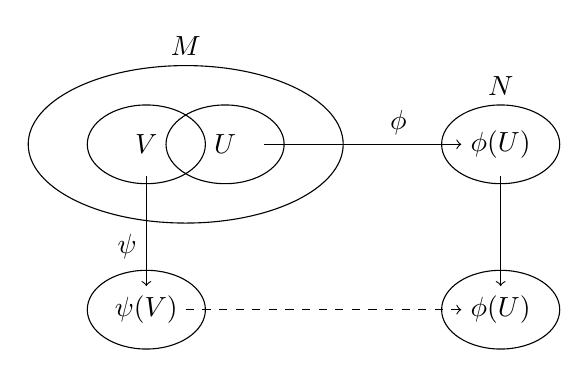
\begin{tikzpicture}
              \draw (-2,2) ellipse (2cm and 1cm);
              \draw (-2.5,2) ellipse (0.75cm and 0.5cm);
              \draw (-1.5,2) ellipse (0.75cm and 0.5cm);
              \node at (-2.5,2) {$V$};
              \node at (-1.5,2) {$U$};
              \node[above] at (-2,3) {$M$};
              \draw[->] (-1, 2) -- (1.5,2);
              \node[above] at (0.7,2) {$\phi$};
              \draw (2,2) ellipse (0.75cm and 0.5cm);
              \node at (2,2) {$\phi(U)$};
              \node[above] at (2,2.5) {$N$};
              \draw[->] (2,1.6) -- (2,0.2);
              \node[right] at (2,1) {$\id$};
              \draw (2,-0.1) ellipse (0.75 cm and 0.5 cm) node {$\phi(U)$};
              \draw[->] (-2.5,1.6) -- (-2.5,0.2);
              \node[left] at (-2.5, 0.7) {$\psi$};
              \draw (-2.5,-0.1) ellipse (0.75 cm and 0.5 cm) node {$\psi(V)$};
              \draw[->,dashed] (-2,-0.1) -- (1.5,-0.1);
        \end{tikzpicture}\]
            Гладкость карты, как диффеоморфизма, эквивалентна тому, что карта согласована с остальными в атласе: пунктирная стрелка $\psi(U \cap V) \map \phi(U \cap V)$ одновременно является и отображением перехода между картами $(U, \phi)$ и $(V, \psi)$, и координатным представлением $\phi$ в картах $(V, \psi), (U, \id)$.
        }
    }
    \corollary{Диффеоморфизм $f: M \map N$ задаёт естественную биекцию между картами $M$ и картами $N$ (а ещё между (максимальными) атласами $M$ и (максимальными) атласами $N$). }
    \newlection{21 февраля 2024 г.}
    \example[Диффеоморфизм]{
        Ранее приводились неэквивалентные карты $(\R, \id)$ и $(\R, [x \mapsto x^3])$.
        Вещественные прямые с данными картами диффеоморфны: $[x\mapsto x^3]$ --- диффеоморфизм, ему обратный $\left[x \mapsto \sqrt[3]{x}\right]$ $\left(\textrm{где, как в школе, }\sqrt[3]{x} = \all{\sqrt[3]{x},&x \ge 0 \\ -\sqrt[3]{-x},&x < 0}\right)$.
    }
    Таким образом, создать две недиффеоморфные структуры на одном и том же многообразии не то чтобы просто.
    \intfact{
    Пусть $M$ --- $n$-мерное многообразие.

        Если $\all{n < 4,&\text{на нём существует единственная гладкая структура} \\ n = 4,&\text{на нём существует бесконечно много гладких структур} \\ n>4,&\text{на нём существует конечное число гладких структур}}$.

        В частности, при $n > 4$: если $M^n = \R^n$, то гладкая структура единственна.
    }
    \subsection{Касательное пространство}
    Пусть $M$ --- гладкое многообразие, $p \in M$.
    Пусть $\alpha, \beta: (\eps, +\eps) \map M$ --- гладкие (естественно, в смысле отображения многообразий) кривые, такие, что $\alpha(0) = p = \beta(0)$.
    \definition[$\alpha$ и $\beta$ соприкасаются в $p$]{
        В любой карте $(U, \phi)$ (где $U \ni p$) их производные в нуле совпадают: $(\phi \circ \alpha)'(0) = (\phi \circ \beta)'(0)$.
    }
    \precaution{
    Определение требует совпадение векторов скорости, а не просто параллельности или сонаправленности.
    }
    \properties[Соприкасающиеся кривые]{
    \item Соприкасаемость кривых в какой-то конкретной точке --- отношение эквивалентности.
    \item Соприкасаемость не зависит от выбора карты: достаточно проверить в любой одной, содержащей $p$.
    \provehere{
        Пусть $(U, \phi)$, $(V, \psi)$ --- две карты, содержащие точку $p$, отображение $f_{\phi\psi} = \psi\circ\phi^{-1}$ гладкое, значит, оно переводит равные векторы в равные.
    }
    }
    \definition[Касательный вектор в точке $p \in M$]{
    Класс эквивалентности соприкасающихся в точке $p$ кривых.
    }
    Множество всех касательных векторов --- \emph{касательное пространство}, обозначают $T_p M$.
    \subsubsection{Координаты касательного вектора}
    Пусть $p \in M$, и $(U, \phi)$ --- карта, содержащая $p$.
    \definition[Координатное представление вектора $v = \lbrack\alpha\rbrack \in T_p M$]{
        Вектор скорости данной кривой в данной карте $v_\phi \bydef (\phi \circ \alpha)'(0)$.
    }
    Понятно, что определение не зависит от выбора представителя --- кривой $\alpha$.

    Также координаты $v_\phi$ в $\R^n$ называют \emph{координатами $v$ в карте $\phi$}.
    \properties[Координатное представление]{
    \item $\forall p \in M, \forall (U, \phi): p \in U \then$ координатное представление --- биекция $\begin{aligned}T_p M &\map \R^n \\ v &\mapsto v_\phi\end{aligned}$.
    \provehere{
    Это инъекция, так как если образы $u, v$ равны, то по определению $u$ и $v$ соприкасаются.

        Это сюръекция: $\forall w \in \R^n$ можно рассмотреть кривую $\gamma(t) \coloneqq w t + \phi(p)$.
        Координаты $[\phi^{-1} \circ \gamma]$ в карте $\phi$ как раз окажутся равными $w$.
    }
    }
    \subsubsection{Преобразование координатного представления в зависимости от карты}
    \statement{\label{change-map}
        Пусть $M^n \ni p$ --- гладкое многообразие и точка, $(U, \phi)$ и $(V, \psi)$ --- карты, содержащие $p$. Тогда $v_\psi = \d_{\phi(p)}{f_{\phi\psi}}(v_\phi)$.
        \provehere{
            Пусть $v = [\alpha]$. Тогда $v_\phi = (\phi \circ \alpha)'(0)$, $v_\psi = (\psi \circ \alpha)'(0)$, и действительно, так как $f_{\phi\psi} = \psi\circ\phi^{-1}$, то $v_\psi = (f_{\phi\psi} \circ \phi \circ \alpha)'(0)$.
            Дифференцируя композицию, получаем утверждение.
        }
    }
    Следствием данного утверждения является альтернативное определение касательного вектора:
    \definition[Касательные векторы в точке $p \in M$]{
    Отображение из множества всех карт, содержащих точку $p$ (обозначим их $\mathcal{M}_p$) в $\R^n$
    \[\mathcal{M}_p \map \R^n\]
    такое, что выполнены соотношения~(\cref{change-map}).
    }
    Это определение сродни тому определению тензора, которое говорит: <<Тензор --- это многомерная матрица чисел, преобразующихся при замене базиса следующим образом\dots>>
    \subsection{Структура векторного пространства на $T_p M$}
    Зафиксируем $p \in M$, и карту $(U, \phi)$, содержащую $p$. Пусть $v, w \in T_p M$.
    \definition[Сумма векторов $v$ и $w$]{ Такой вектор $v + w$, что $(v + w)_\phi = v_\phi + w_\phi$.}
    \definition[Растяжение вектора $v$ с коэффициентом $\alpha$]{ Такой вектор $\alpha v$, что $(\alpha v)_\phi = \alpha \cdot v_\phi$.}
    Иными словами, у нас была биекция $T_p M$ с векторным пространством, и мы просто перенесли структуру векторного пространства с $\R^n$ на $T_p M$.
    Определение не зависит от выбора карты, так как замена координат касательных векторов при переходе между картами --- изоморфизм векторных пространств (дифференциал --- линейный оператор).
    \note{
        Из определения получается, что $v \map v_\phi$ --- изоморфизм векторных пространств.
    }
    \section{Касательное расслоение}
    Как множество, $T(M) = \bigsqcup\limits_{p \in M}T_p M$.
    Оказывается, на $T(M)$ можно естественно ввести топологию и гладкую структуру размерности $2n$.
    Преобразуем определение атласа так, чтобы это случилось одновременно.

    \statement[Атлас для множества]{
        Пусть $X$ --- множество с картами $(U, \phi)$, то есть парами $(U, \phi)$ где $U \subset X$, и каждая $\phi$ --- биекция $U \map \R^n$. При этом $X = \bigcup U$

        Потребуем для любых двух карт $(U, \phi)$ и $(V, \psi)$: $\phi(U \cap V)$ открыто (в частности, $\phi(U)$ открыто), и потребуем, чтобы все функции перехода $f_{\phi\psi} = \psi \circ \phi^{-1}$ были гладкими.

        Введём на $X$ топологию: $W \subset X$ открыто, если $\forall (U, \phi): \phi(U \cap W)$ открыто, и предположим, что топология получилась хаусдорфовой, и на $X$ есть счётная база.

        Тогда утверждается, что данная процедура задаёт на $X$ одновременно и топологию, и гладкую структуру.
    }
    Зададим такую гладкую структуру на $T(M)$.
    Обозначим $T U = \bigsqcup\limits_{p \in U}T_p M$.
    Можно рассматривать $TU = \defset{(p, v)}{p \in U, v \in T_p M}$.

    Пусть имеется карта $(U, \phi)$ на $M$.
    Построим по ней карту \begin{align*}\Phi: TU &\map \R^n \times \R^n \\ (p, v) & \mapsto (\phi(p), v_\phi)\end{align*}

    Проверим согласованность: пусть $(U, \phi)$ и $(V, \psi)$ --- две карты на $M$.
    По ним построены карты $(TU, \Phi)$ и $(TV, \Psi)$ соответственно.
    Тогда $(\Psi \circ \Phi^{-1})(p, v) = ((\psi \circ \phi^{-1})(p), \d_{\phi(p)}{f_{\phi\psi}}(v))$, видно, что $\Psi \circ \Phi^{-1}$ гладко.

    \exercise{
    Получилось хаусдорфовое пространство со счётной базой.
    }
%    \comment{На лекции леммы ниже не было, но давайте для порядка докажем. Проверка свойств всё равно остаётся читателю в качестве упражнения.}
%    \lemma{
%        Получилось хаусдорфово пространство со счётной базой.
%        \provebullets{
%        \item Проверим хаусдорфовость. Рассмотрим две точки $(p_1, v_1), (p_2, v_2) \in TM$.
%
%            Пусть $p_1 \ne p_2$. Выберем карты $(U_1, \phi_1)$ и $(U_2, \phi_2)$, где $p_i \in U_i$.
%            Так как $M$ хаусдорфово, а атлас максимальный, то можно считать, что $U_1 \cap U_2 = \o$ (при необходимости уменьшить $U_1$ и $U_2$).
%            Множества $T U_1$ и $T U_2$ открыты в $TM$ и являются непересекающимися окрестностями $p_1$ и $p_2$.
%
%            Теперь пусть $p_1 = p_2$, $v_1 \ne v_2$. Выберем карту $(U, \phi)$, где $p \in U$, по ней построена карта $(TU, \Phi)$.
%            Из хаусдорфовости $\R^n$ найдётся непересекающиеся окрестности $v_1$ и $v_2$, пусть это $V_1$ и $V_2$ соответственно.
%
%            Тогда $\Phi^{-1}(V_1)$ и $\Phi^{-2}(V_2)$ --- непересекающиеся окрестности $(p_1, v_1)$ и $(p_2, v_2)$.
%        \item Пусть на $M$ имеется счётная база $\{U_i\}_{i \in I}$, возьмём в $\R^n$ какую-то счётную базу $\{V_j\}_{j \in J}$.
%
%            Пусть $\mathcal{U} \coloneqq \defset{U_i}{i \in I, \exists \phi_i: (U_i, \phi_i)\text{ --- карта}}$.
%            В следующем абзаце покажем, что $\mathcal{U}$ --- тоже (понятно, счётная) база.
%
%            Рассмотрим произвольное открытое $U \subset M$, и $p \in U$. Пусть имеется карта $\left(\tilde{U}, \tilde{\phi}\right)$, содержащая $p$, тогда $U \cap \tilde{U}$ открыто, и по критерию базы имеется $U_i$ ($i \in I$), такое, что $p \in U_i \subset U \cap \tilde{U}$.
%            Так как атлас максимален, то $\left(U_i, \tilde{\phi}\big|_{U_i}\right)$ --- карта.
%
%            Раз $\mathcal{U}$ --- счётная база, то считаем, что эта база совпадает с $\{U_i\}_{i \in I}$.
%            Пусть по карте $(U_i, \phi_i)$ построена карта $(T U_i,\Phi_i)$, тогда $\{\Phi_i^{-1}(\phi_i(V_j))\}_{i \in I, j \in J}$ --- счётная база в $TM$.
%        }
%    }
    \subsection{Дифференциал гладкого отображения}
    Пусть $M$ и $N$ --- гладкие многообразия, и есть гладкое отображение $f: M \map N$.
    Зафиксируем $p \in M$.
    \definition[Дифференциал $f$ в точке $p$]{
    Отображение $\d_p f: T_p M \map T_{f(p)}N$, заданное следующим образом: $\d_p f: [\alpha] \mapsto [f \circ \alpha]$.
    }
    \statement{
        Определение дифференциала не зависит от выбора представителей.
        \provehere{
            Пусть $\alpha \sim \beta$ --- две кривые, $\alpha(0) = \beta(0) = p$, $\alpha'(0) = \beta'(0) = v$.

            Проверим, что $f \circ \alpha \sim f \circ \beta$.
            Достаточно проверить, что совпадают координатные представления.

            Выберем две карты $(U, \phi)$ и $(V, \psi)$ (где $U \ni p$, $V \ni f(p)$).
            Координатное представление $f$ --- это $\tilde{f} = \psi \circ f \circ \phi^{-1}$.

            Дифференциал $\tilde{f}$ переносит координаты представления векторов из $T_p M$ в координаты представления векторов из $T_{f(p)}N$:
        \gather{\psi \circ f \circ \alpha = \tilde{f} \circ \phi \circ \alpha \text{\quadи\quad}\psi \circ f \circ \beta = \tilde{f} \circ \phi \circ \beta\\ (\psi \circ (f \circ \alpha))'(0) = \d_{\phi(p)} \tilde{f}((\phi \circ \alpha)'(0)) = \d_{\phi(p)} \tilde{f}((\phi \circ \beta)'(0)) = (\psi \circ (f \circ \beta))'(0)\qedhere }
        }
    Нетрудно заметить, что $(\d_p f(v))_\psi = \left(\d_{f(p)}\tilde{f}\,\right)(v_\phi)$ в обозначениях из доказательства выше (и $v = [\alpha]$).
    \corollary{
        $\d_p f$ --- линейное отображение.
    }
    }
    \newlection{28 февраля 2024 г.}
    \note{
    Можно естественным определить дифференциал на всём пространстве $T f: T M \map T N$.
        На вектор $v \in T_p M$ $T f$ действует понятным образом: $v \mapsto \d_p f(v)$.
    }
    Если $U \subset \R^n$, то касательное пространство $TU$ естественным образом отождествляется с $U \times \R^n$.
    \section{Гладкие векторные поля}
    Пусть $M$ --- гладкое многообразие, выберем произвольное подмножество $A \subset M$.

    \definition[Непрерывное векторное поле на $A$]{
        Непрерывное отображение $X: A \map TM$, такое, что $\forall p \in A: X(p) \in T_p M$.
    }
    \definition[Гладкое векторное поле на $A$]{
        Векторное поле $X: A \map TM$, такое, что $\exists$ открытое $U \subset M: U \supset A$, и $X$ продолжается на $U$, как гладкое векторное поле (то есть гладкое отображение, являющееся непрерывным векторным полем).
    }
    Для гладкого многообразия $M$ будем обозначать пространство всех гладких векторных полей за $\mathscr{X}(M)$.

    Пусть в $M$ имеется карта $(U, \phi)$.
    \definition[Координатное векторное поле, соответствующее $i$-й координате]{
        Векторное поле $V_i: U \map TM$, такое, что $\d \phi(V_i) = e_i$ ($V_i(p) = e_i$) \comment{Или что-то похожее, я не очень понял}
    }
    \lemma{
        Пусть имеется открытое $U \subset \R^n$, и компактное $K \subset U$.
    Утверждается, что $\forall V \supset K: \Cl V \subset U \then$ можно построить гладкую функцию $f: \R^n \map \R$, такую, что $f\big|_{K} = 1$, $f\big|_{\R^n \sm V} = 0$.
    \provehere{
    \comment{На лекции шло без доказательства.}
    %$\R^n \sm V$ замкнуто, $d \coloneqq \dist(\R^n \sm V, K) > 0$, свернём $\chi todo$
    }
    }
    \corollary{
        Пусть $V_i$ --- координатное поле карты $(U, \phi)$.
        Тогда $\forall K \subset U: \exists$ векторное поле $\tilde{V}_i: \tilde{V}_i\big|_{K} = V_i, \tilde{V}_i\big|_{M \sm U} \equiv 0$.

    Иными словами, всегда немного уменьшив карту, можно продолжить координатное векторное поле на всё многообразие.
    }
    \section{Гладкие подмногообразия}
    Пусть $M^m$ --- гладкое многообразие размерности $m$.
    \definition[Гладкое подмногообразие размерности $n \le m$]{
    Подмножество $N \subset M$, такое, что $\forall x \in N: \exists$ выпрямляющая карта $(U, \phi)$ (карта на $M$), такая, что $U \ni p$ и $\phi(U) \cap \R^n = \phi(N \cap U)$.
    }
    Здесь имеется в виду, что $\phi$ действует в $\R^m$, где как-то введены координаты, и имеется определённое вложение $\R^n \hookrightarrow \R^m$.
    \statement{
    На $N$ каноническим образом индуцируется гладкая структура из $M$. Карты на $N$ --- сужения выпрямляющих карт (карте $(U, \phi)$ отвечает карта $N \cap U, \psi$, где $\psi: N \cap U \map \R^n \subset \R^m$, $\psi(x) = \phi(x)$).
    \provehere{
    Согласованность карт на $N$ следует из согласованности карт на $M$.
    }
    }
    Пусть $N^n, M^m$ --- гладкие многообразия.
    \definition[Погружение $f: N \map M$]{
    Гладкое отображение $f: N \map M$, такое, что $\forall p \in N: \d_p f$ --- инъекция.
    Само $f$ не обязано быть инъекцией.
    }
    Понятно, что такое возможно только при $n \le m$.
    \definition[Вложение $f: N \map M$]{
        Погружение $f: N \map M$, которое является топологическим вложением, то есть гомеоморфизмом на образ.
    }
    \examples{
    \item В случае поверхностей размерности $2$ погружение подмногообразия размерности $1$ --- кривой --- называлось регулярной параметризацией.
    \item Петля слева является погружением, но даже инъективная петля справа вложением не является: в выделенной точке топология не совпадает с топологией интервала.
        \[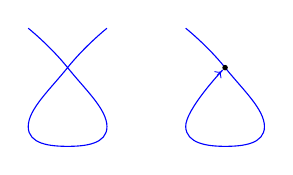
\begin{tikzpicture}
              \draw[blue] plot [smooth,tension=0.8] coordinates {(-0.5,0.5) (0,0) (0.5,-0.75) (0,-1) (-0.5,-0.75) (0,0) (0.5,0.5)};
              \draw[blue] plot [smooth,tension=0.8] coordinates {(1.5,0.5) (2,0) (2.5,-0.75) (2,-1) (1.5,-0.75) (1.97,-0.03)};
              \draw[blue,->] (1.9,-0.1) -- (1.95,-0.05);
              \fill (2,0) circle (1pt);
        \end{tikzpicture}\]
    }
    \proposal{\down
    \numbers{
        \item Погружение локально является вложением: $\forall x \in N: \exists U_x \ni x: f\big|_{U_x}$ --- вложение.
        \item Образ вложения --- гладкое подмногообразие.
    }
    \comment{
        С доказательством этого очевидного предположения возникли неожиданные проблемы, я что-то написал ниже, за правильность не ручаюсь.
    }
    \provehere {
        Достаточно доказать для случая открытых $N \subset \R^n$, $M = \R^m$, потому что карты --- диффеоморфизмы, и определения сохраняются при диффеоморфизмах.

        Зафиксируем $x \in N$.
        Введём координаты в $\R^m$, выделив первые $n$ координат, так, чтобы подпространство, натянутое на них, совпадало с $\d_x f(\R^n)$.

        Также домножим пространство, содержащее $N$, на $\R^{m - n}$.
        \indentlemma{
            Существует $W \ni x, W' \ni f(x), \phi: W \map W': \phi\big|_{N \cap W} = f$ ($W \in \R^m, W' \in \R^m$).
        }{
            Обозначим координаты в $\R^n \times \R^{m-n}$ за $(\xi, \zeta)$, и определим $\phi(x + \xi, \eta) = f(x) + f(\xi) + (0, \eta)$.
        Действительно, дифференциал $\d_x\phi = (\d f, \id)$ невырожден.

        По теореме об обратной функции $\exists W: \phi\big|_W$ --- диффеоморфизм.
        }
    \numbers{
    \item Образ $f\big|_{N \cap W}$ --- подмногообразие $W \cap \R^n \subset N$. $\phi^{-1}\big|_{W'}$ --- выпрямляющая карта,
    \item $\phi$ --- гомеоморфизм на образ $\then f\big|_{N \cap W}$ --- топологическое вложение и гомеоморфизм.
        Значит, локально погружение --- вложение.
    \item Так как $f$ --- топологическое вложение, то $f(N)$ --- подмногообразие.
    }
    }
    }
    \newlection{6 марта 2023 г.}
    \counterexample{
        Тождественное отображение между прямыми $(\R, x^3) \map (\R, \id)$ --- не вложение (и даже не погружение).
    }
    Пусть $N \subset M$ --- гладкое подмногообразие.
    Отображение $\text{in}: N \hookrightarrow M$ можно рассматривать, как вложение многообразия.

    \statement{
    Следующие определения подмногообразия равносильны:
    \bullets{
    \item Подмножество $N \subset M$ с выпрямляющими картами.
    \item Образ вложения некоторого многообразия.
    }
    }
    \intfact[Теорема Уитни]{
    Для любого гладкого многообразия $M^m$ существует вложения $M^m \hookrightarrow \R^{2m}$.
    }
    \section{Риманова геометрия}
    Пусть дано гладкое многообразие $M^m$.
    \definition[Риманова структура на $M^m$]{
        Совокупность (положительно определённых) скалярных произведений $\{g_x\}_{x \in M}$ ($g_x: T_x M \times T_x M \map \R, g_x = \angles{\_, \_}_x)$).
        Иначе это называют \emph{метрическим тензором}.
    }
    Напомним, что $\mathscr{X}(M)$ --- пространство гладких векторных полей на $M$.
    \definition[Гладкая риманова структура на $M^m$]{
    Такая риманова структура, что ${\forall X, Y \in \mathscr{X}(M)}: \begin{aligned}M &\map \R \\ x &\mapsto \angles{X_x, Y_x}_x\end{aligned}$ гладко
    }
    Далее везде будем говорить \emph{риманово многообразие} для многообразия с гладкой римановой структурой.
    \example{
    Пример (гладкого) метрического тензора для поверхностей --- первая квадратичная форма.
    }
    Пусть заданы два римановых многообразия $(M_1, g_1)$ и $(M_2, g_2)$.
    \definition[Изометрия между $M_1$ и $M_2$]{
    Диффеоморфизм $f: M_1 \map M_2$, сохраняющий скалярные произведения: $\forall x \in M_1: \forall v, w \in T_x M_1: \angles{v, w} = g_{f(x)}(\d_x f(v), \d_x f(w))$.
    }
    \examples{
        \item Пусть имеется вложение гладкого многообразия $f: M^m \map \R^n$.
        В соответствии с ним на $M^m$ можно естественным образом задать риманову метрику: \[\forall x \in M: \forall v, w \in T_x M: \angles{v, w}_x \coloneqq \angles{\d_x f(v), \d_x f(w)}_{f(x)}\]
    Так как $\d_p f$ инъективен, то скалярное произведение получится невырожденным.

        В предыдущем семестре в точности это происходило с вложением поверхности в $\R^3$.
        \item Пусть на многообразии $N^n$ задана риманова структура, и имеется вложение $f: M^m \map \R^n$.
            Тогда абсолютно аналогично можно задать риманову метрику на $M^m$:
        \[\forall x \in M: \forall v, w \in T_x M: \angles{v, w}_x \coloneqq \angles{\d_x f(v), \d_x f(w)}_{f(x)}\]
    \item В обеих пунктах можно ослабить требования на $f$: достаточно, чтобы $f$ было погружением.
    }
    Пусть $(M^m, g)$ --- риманово многообразие, $(U, \phi)$ --- карта: $\phi: U \map \phi(U) \subset \R^m$.
    Выберем в $\R^m$ ортонормированный базис $(e_i)_{1 \le i \le m}$.
    Базисный вектор $e_i$ --- координатное представление вектора $\d_x\phi^{-1}(e_i)$, и $(\d_x\phi^{-1}(e_i))_{1 \le i \le m}$ --- базис $T_x M$.

    Значит, можно записать координаты метрического тензора $g_x$ в данных базисных векторах $\d_x \phi^{-1}(e_i)$, получатся \emph{метрические коэффициенты для карты $(U, \phi)$}: $(g_{i,j})_{1 \le i,j \le m}$.
    Для векторов $X = X_1 \d_x\phi^{-1}(e_1) + \dots + X_m \d_x \phi^{-1}(e_m)$ и $Y = Y_1 \d_x\phi^{-1}(e_1) + \dots + Y_m \d_x \phi^{-1}(e_m)$: $\angles{X, Y} = \sum\limits_{i,j}X_i g_{i,j} Y_j$.

    \theorem{
    $g_{i,j}$ --- гладкие во всех картах $\iff$ метрический тензор $g$ гладок.
    \provewthen{
        \comment{Не успел нормально записать}
    Рассмотрим карту $(U, \phi)$.

    В определении гладкого метрического тензора были $X, Y \in \mathscr{M}$, но на прошлой лекции мы обсудили, что можно считать, что для компакта $K \subset U$, сколь угодно близкого приближающего $U$,...
    $g(\overline{X}_i, \overline{Y}_i)$ --- гладкая функция, совпадает с $g_{i,j}$ на компакте.

    Проверяем гладкость в какой-то конкретной точке, точку можно захватить компактом, получается, верно для всех точек.
    }{
        Рассмотрим гладкие векторные поля $X, Y \in \mathscr{X}(M)$.

        Проверим гладкость в точке $x \in M$.
        Рассмотрим произвольную карту $(U, \phi)$, содержащую $x$,
        Распишем $X = \sum\limits_{i}\xi_i X_i, Y = \sum\limits_{j}\eta_j X_j$.
        Понятно, что $\xi_i, \eta_j: M \map \R$ --- гладкие функции.

        Получается, $\angles{X, Y}_x = \sum\limits_{i,j}\xi_i \eta_j \angles{X_i, X_j} = \sum\limits_{i,j}\xi_i \eta_j g_{i,j}$.
    }
    }
    \example{
        Пусть многообразие $M^m$ покрыто одной картой $(M, \phi)$.
        Можно ввести $m \times m$ гладких метрических коэффиицентов $g_{i,j}: M \map \R$ так, что матрица $(g_{i,j})$ всюду положительно определена.

        В случае покрытия $M$ несколькими картами так может не получиться, надо ещё проверять согласованность, что может быть неудобно.
    }
    Аналогично поверхностям, определим длину путей.

    Пусть $v \in T_x M$.
    \definition[Длина вектора $v$]{ $|v| \bydef \sqrt{\angles{v, v}_x}$. }
    Теперь $\gamma: [a, b] \map M$ --- кусочно-гладкая кривая (имеется разбиение $a = t_0 \le t_1 \le \dots \le t)n = b$, такое, что $\gamma\big|_{[t_i,t_{i+1}]}$) --- гладкая.
    \definition[Длина кривой]{
        $L(\gamma) = \sum\limits_{i}\int\limits_{t_i}^{t_{i+1}}|\gamma'(t)|\d t$.
        Длина $\gamma'$ определена: из гладкости $\forall t \in (t_i, t_{i+1}): \gamma'(t) \in T_{\gamma(t)}M$.
    }
    Пусть $(M, g)$ --- связное риманово многообразие, $x, y \in M$ --- две точки.
    \definition[Расстояние между точками $x, y$]{
    $d_l(x, y) \bydef \inf_{\gamma} l(\gamma)$, где инфимум берётся по всем кусочно гладким $\gamma: [a, b] \map M$, таким, что $\gamma(a) = x, \gamma(b) = y$.
    }
    \theorem{\down
    \numbers{
    \item $d_l$ --- метрика
    \item Топология, порождённая $d_l$ совпадает с исходной топологией $\Omega M$.
    }
    \provenumbers{
    \item Проверим три аксиомы метрики.
    \bullets{
    \item Меняя направление пути, получаем $d_l(x, y) = d_l(y, x)$.
    \item Выберем $\eps > 0$, найдутся две кусочно гладкие кривые $\gamma_{x,y}$ и $\gamma_{y,z}$, почти оптимально соединяющие $x,y$ и $y,z$ соответственно ($l(\gamma_{x,y}) \le d(x, y) + \eps;\: l(\gamma_{y,z}) \le d(y, z) + \eps$).
    Конкатенируя $\gamma_{x,y}\cdot \gamma_{y,z}$, получаем $d_l(x, z) \le d_l(x, y) + d_l(y, z) + 2\eps$.
        Устремляя $\eps \to 0$, получаем неравенство треугольника.
    \item Проверим положительную определённость.
    \indentlemma{\label{strong-equivalence}
    $\forall x \in M: \exists$ карта $(U, \phi)$, содержащая $x$, такая, что $\forall \eps > 0: \exists V \subset U$ ($V \ni x$), причём $\phi\big|_V: V \map \phi(V)$ $(1\pm\eps)$-билипшицево:
    \[\forall a, b \in V: (1 - \eps)|\phi(a) - \phi(b)| \le d_l(a, b) \le (1 + \eps)|\phi(a) - \phi(b)|\]
    Отсюда сразу получается, что $\forall \gamma: [c, d] \map V$:
        \[(1 - \eps) \cdot l(\phi \circ \gamma) \le l(\gamma) \le (1 + \eps)\cdot l(\phi \circ \gamma)\]
    }{
        Выберем ортонормированный базис $X_1, \dots, X_m$ в $T_x M$ (такой найдётся, так как скалярное произведение положительно определено).

        Выберем произвольную карту $(U, \phi)$, содержащую $x$. $\d_x\phi(X_1), \dots, \d_x\phi(X_m)$ --- базис в $\R^m$, его можно линейным преобразованием $L$ перевести в ортонормированный.
        Далее считаем, что он уже ортонормирован (можно заменить карту $\phi$ на $T \circ \phi$).

        Коэффициенты метрического тензора в этой карте $g_{i,j}$ таковы, что $g_{i,j}(x) = \delta_{i,j}$.

        Из непрерывности $g_{i,j}: \forall \eps > 0:\exists \underset{\ni x}V \subset U: \forall y \in V, v \in T_y M: {|\d_x\phi(v)| = (1 \pm \eps)|v|}$.

    }
    }
    \item Применяем~(\cref{strong-equivalence}) для $\eps = \nicefrac{1}{2}$.
        Из билипшицевости сразу получается совпадение топологий.
    }
    }
    \subsection{Отсупление в метрические пространства}
    Более частым случаем является определение расстояние, как инфимум длин всех кривых, а не только кусочно-гладких.

    Пусть $(X, d)$ --- метрическое пространство, $\gamma: (c, d) \map X$ --- (непрерывный) путь.
    Здесь длина определяется по формуле $L_d(\gamma) = \sup\sum\limits_{i}d(\gamma(t_i), \gamma(t_{i+1}))$, где супремум берётся по всем разбиениям $c = t_0 \le t_1 \le \dots \le t_n = d$.
    \definition[Спрямляемая кривая $\gamma$]{ $L_d(\gamma) < \infty$.}
    Пусть $x, y \in X$.
    \definition[Внутренняя метрика, порождённая метрикой $d$]{
    $d_I(x, y) \bydef \inf_{\gamma} l(\gamma)$, где инфимум берётся по всем кусочно гладким $\gamma: [a, b] \map M$, таким, что $\gamma(a) = x, \gamma(b) = y$.
    }
    Из неравенства треугольника $d_I \ge d$.
    \intfact{
        $(d_I)_I = d_I$.
    }
    \definition[Внутренняя метрика]{
        Метрика $d$, совпадающая с внутренней метрикой, порождённой $d$.
    }
    \example[Не внутернняя метрика]{
    Рассмотрим окружность $S^1 \subset \R^2$.
        Метрика, индуцированная с $\R^2$ на $S^1$ --- не внутренняя.
    }
    \intfact{
        $d_l$ --- внутренняя метрика, и $l = L_{d_l}$.
    }
    Для доказательства стоит использовать~(\cref{strong-equivalence}).
    \newlection{13 марта 2023 г.}
    //todo
    \newlection{20 марта 2024 г.}
    \subsection{Аксиомы плоскости Лобачевского}
    <<На самом деле, аксиом много, и их можно по-разному выбирать>>

    Аксиомы аналогичны евклидовым.
    \numbers{
    \item Через любые две точки проходит единственная прямая.
    \item Прямая разбивает плоскость на две части: любой отрезок, соединяющий две точки, пересекает данную прямую не более, чем в одной точке, и точки бьются на два класса эквивалентности относительно данного отношения.
    \item Аксиома параллельных не верна: через одну точку можно провести много прямых, параллельных данной (не пересекающих данную):
        \[\begin{tikzpicture}
            \draw (0, 0) -- (0, 2) node[above right] {$l$};
            \fill (1.5, 0.5) circle (1pt) node[above right] {$p$};

            \draw (2, 0) circle ({sqrt(2)/2});
            \draw (1, 0) circle ({sqrt(2)/2});
            \draw (1.5, 0) -- (1.5, 2);
            \fill[white] (0, 0) rectangle (2.9, -1);
            \draw[->] (-1, 0) -- (3, 0) node[above right]{$x$};

        \end{tikzpicture}\]

    \intfact{Это равносильно тому, что не существует точки $O$, в которой можно произвести гомотетию: $d(\lambda A, \lambda B) \ne \lambda d(A, B)$.}
    \item Однородность движения.
    \definition[Флаг]{Тройка из точки, луча и полуплоскости, расположенных так:
    \[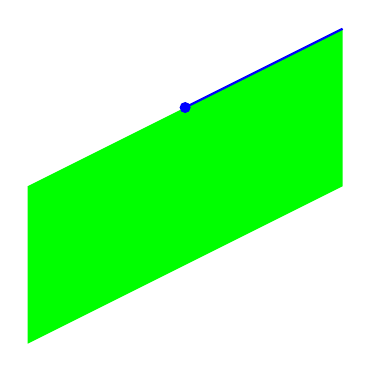
\begin{tikzpicture}
          \fill[green] (-2,-1) -- (2,1) -- (2, -1) -- (-2,-3) -- cycle;
          \draw[blue,thick] (0, 0) -- (2, 1);
          \fill[blue] (0,0) circle (2pt);
    \end{tikzpicture}\]
    }
    Любой флаг переводится в любой другой движением.

    Докажем, что данная аксиома верна в нашей модели.
    \provehere{
    Достаточно доказать, что в данный флаг можно перевести любой другой.

    В качестве фиксированного флага выберем [$(0, 1)$, вверх, вправо].

    Далее инверсия, сдвиг, отражение.
    }
    \item Неравенство треугольника: $d(x, y) \le d(x, z) + d(z, y)$, и равенство имеет место только когда $z \in [x, y]$.
    }
    \comment{И вот прямо такая маленькая система аксиом задаёт плоскость Лобачевского? Я забыл спросить }
    \section{Модель Пуанкаре в круге}
    Сделаем инверсию $I$ модели Лобачевского относительно $A = (0, -1)$ с коэффициентом $K = \sqrt{2}$.

    $\angles{v, w}_{H_P} = \angles{\d I(v), \d I(w)}_{H_L}$.

    Метрика осталась конформной, роль прямых теперь играют диаметры и ортогональные дуги окружностей.
    \theorem{
    Конформный фактор метрики равен $\frac{2}{1 - x^2 - y^2}$.
    Иными словами, для $v \in T_{(x, y)}H_P: |v|_{H_P} = \frac{2}{1 - x^2 - y^2}|v|_E$.
    \provehere{
    Рассмотрим $(x_0, y_0) \in H_P$.
        Пусть $(x_1, y_1) = I(x_0, y_0)$.
        Конформный фактор гиперболической плоскости в модели Лобачевского в точке $(x_1, y_1)$ равен $\frac{1}{y_1}$.

        Пусть при инверсии с центром в точке $A$ точка $B$ переходит в $B'$.
        Тогда имеется равенство $\dir{AB} = \dir{AB'}\frac{R^2}{|AB'|^2|}$.
        Выразим $y_1$ через $x_0, y_0$:
        \[y_1 = -1 + (y_0 + 1) \cdot \frac{2}{x_0^2 + (y_0 + 1)^2} = \frac{-x_0^2 - y_0^2 + 1}{r^2}\]
    С другой стороны, конформный фактор инверсии равен $\lambda_I = \frac{2}{r^2}|v|_E$.

        Получаем $|\d_{(x_0, y_0)} I(v)|_{H_L} = \frac{|\d I(v)|_E}{y_1} = \frac{2}{1 - x_0^2 - y_0^2}$.

    Матрица Грама имеет вид $\vect{\frac{4}{(1 - x^2 - y^2)^2}&0\\0&\frac{4}{(1 - x^2 - y^2)^2}}$.
    }
    }
    \section{Касательный вектор как дифференцирование}
    Пусть $M$ --- гладкое многообразие. $\mathscr{F}(M)$ --- множество гладких функций, $\mathscr{X}(M)$ --- множество гладких векторных полей.

    Естественным образом, $\mathscr{F}(M)$ и $\mathscr{X}(M)$ образуют векторные пространства над $\R$.
    При этом, на $\mathscr{X}(M)$ также есть поточечное умножение, и $\mathscr{F}(M)$ таким образом формируют ассоциативную, коммутативную $\R$-алгебру.
    При этом $\mathscr{X}(M)$ также является модулем над $\mathscr{F}(M)$. \comment{Видимо, относительно поточечного умножения}.

    Как известно из курса алгебры, дифференциальный оператор $D$ на $\R$-алгебре $A$ --- это такой линейный оператор $D: A \map A$, что выполнено правило Лейбница: $D(f \cdot g) = D(f) \cdot g + f \cdot D(g)$.
    Все дифференцирования образуют $\R$-линейной пространство $\Der(A)$.

    Для алгебры $\mathscr{F}(M)$ всякий $X \in \mathscr{X}(M)$ индуцирует дифференцирование $D_X$:
    \[(D_X(f))(x) = \d_x f(X_x)\]
    Правило Лейбница выполнено, так как оно имеет место при дифференцировании произведения.
    \theorem{
    Выше определённое отображение $\mathscr{X}(M) \map \Der(\mathscr{F}(M))$ является изоморфизмом.
    \provehere{
     \indentlemma{
         Зафиксируем $p \in M$.

        Пусть $\overline{D}: \mathscr{F}(M) \map \R$ --- $\R$-линейное отображение, такое, что $\overline{D}(f \cdot g) = \overline{D}(f) \cdot g(p) + f(p) \cdot \overline{D}(g)$.

    \numbers{
        \item Тогда $\exists ! v \in T_p M: \overline{D} = D_v \bydef [f \mapsto \d_pf(v)]$.

        \item В любой карте $(U, \phi)$: $\tilde{x}_i \bydef x_i \circ \phi$: $v_i = \overline{D}(\tilde{x}_i)$.
    }
    }{
         Заметим, что $\overline{D}(\const) = 0$ (проверим для $1: \overline{D}(1) = \overline{D}(1) \cdot 1 + 1 \cdot \overline{D}(1) = 2\overline{D}(1)$).

         Заметим, что $\overline{D}$ локально: если $f\big|_{U_p} = g\big|_{U_p}$, то $\overline{D}(f) = \overline{D}(g)$.

         Сконструируем такую $h$, что в некоторой окрестности $p: h \equiv 1$, и $h\big|_{M \sm U} \equiv 0$ (шапочка).
         Далее показываем локальность... %Из локальности $\overline{D}(h) = 0$. ???

        Пусть $\phi$ --- карта, $v = (v_1, \dots, v_n)$.
         Заметим, что $D_v(\tilde{x}_i) = v_i$.
         Отсюда следует единственность и 2.

        Теперь докажем существование. Зафиксируем карту. $v_i \coloneqq D(\tilde{x}_i)$.
        \indentlemma[Адамар]{
            Пусть $f \in C^{\infty}(\R^n)$. Тогда $\exists g_1, \dots, g_n$ --- гладкие, такие, что $f(x) - f(0) = \sum\limits_{i}g_i(x) \cdot x_i$.
        }{
            Положим $g_i(x) \coloneqq \int\limits_{0}^{1}\der{f}{x_i}(tx)\d t$.
            Проверим, что всё работает:
        \[f(x) - f(0) = \int\limits_{0}^{1}\frac{\d f(tx)}{\d t}\d t =  \int\limits_{0}^{1}\sum\limits_{i = 1}^{n}\der{f}{x_i}(tx)\cdot x_i \d t = \sum\limits_{i = 1}^{n}g_i(t)\cdot x_i\]
        }
     $\overline{D}(f(0) + \sum\limits_{i}x_i \cdot g_i(x)) = \sum\limits_{i}\overline{D}(x_i \cdot g_i) = \sum\limits_{i}\overline{D}(x_i) \cdot g + x_i \cdot \overline{D}(g)$...
        }
    Отсюда следует сюръективность $\mathscr{X}(M) \map \Der(\mathscr{F}(M))$ --- по $D$ определяем $X(D)$, и проверяем, что получился (гладкий) элемент $\mathscr{X}(M)$.
    }
    }
    \newlection{27 марта 2024 г.}
    \section{Скобка Ли векторных полей}
    Пусть $M$ --- гладкое многообразие, $X, Y \in \mathscr{X}(M)$.
    \definition[Скобка Ли векторных полей]{
        Отображение $[\_, \_]: \mathscr{X}(M) \times \mathscr{X} \map \mathscr{X}$, которое двум полям $X, Y$ сопоставляет векторное поле, соответствующее дифференцированию
        \[X(Y(f)) - Y(X(f))\]
    Иными словами, $[X, Y]f = X(Y(f)) - Y(X(f))$.
    }
    Проверим, что это действительно дифференцирование.
    Линейность очевидна;\ правило Лейбница:
    \multline{X(Y(f)) \cdot g + \cancel{Y(f) \cdot X(g)} + \bcancel{X(f) \cdot Y(g)} + f \cdot X(Y(g)) - Y(X(f)) \cdot g - \bcancel{X(f) \cdot Y(g)} - \cancel{Y(f) \cdot X(g)} - f \cdot Y(X(g)) =\\= X(Y(f) \cdot g + f \cdot Y(g)) - Y(X(f) \cdot g + f \cdot X(g)) = X(Y(f \cdot g)) - Y(X(f \cdot g))= [X, Y](f \cdot g) \overset{?}=\\\overset{?}= ([X, Y]f) \cdot g + f \cdot ([X, Y]g) = (X(Y(f)) - Y(X(f))) \cdot g + f \cdot (X(Y(g)) - Y(X(g)))}
    \subsection{Выражение для скобки Ли в координатах}
    Пусть $X, Y$ --- два гладких векторных поля, $\phi: U \map \Omega$ --- карта.

    Введём $\tilde{x}_i \coloneqq x_i \circ \phi$, запишем
    \[[X, Y]_i = D_{[X, Y]}(\tilde{x}_i) =D_{[X_\phi, Y_\phi]}(x_i) = [X_\phi, Y_\phi]_i = X_\phi Y_\phi(x_i) - Y_\phi X_\phi(x_i) \]
    \subsection{Пространство $\mathscr{X}(M)$ вместе со скобкой Ли образует алгебру Якоби}
    Чтобы проверить, что $\mathscr{X}(M)$ образует алгебру Ли, убедимся, что выполнены три аксиомы алгебр Ли:
    \numbers{
    \item Линейность по обеим аргументам: $\forall \alpha_i, \beta_j \in \R, X, Y \in \mathscr{X}(M)$: \gather{[\alpha_1 X_1 + \alpha_2 X_2, Y] = \alpha_1[X_1, Y] + \alpha_2[X_2, Y] \\ [X, \beta_1 Y_1 + \beta_2 Y_2] = \beta_1[X, Y_1] + \beta_2[X, Y_2]}
    \item Кососимметричность: $[X, Y] = -[Y, X]$, или же (эквивалентно) антисимметричность ${[X, X] = 0}$.
    \item Тождество Якоби $[X, [Y, Z]] + [Y, [Z, X]] + [Z, [X, Y]] = 0$.
    }
    \subsection{Специфичные свойства скобки Ли векторных полей}
    Пусть $f, g \in \mathscr{F}(M)$.
    \properties[Скобка Ли]{
    \item $[fX, Y] = f \cdot [X, Y] - Y(f) \cdot X$.
        \provehere{
        \[[f\cdot X, Y](h) = (f\cdot X)(Y(h)) - Y((f\cdot X)(h)) =(f\cdot X)(Y(h)) - Y(f \cdot X(h))\circlesign{=}\]
        Так как $(f\cdot X)(\cdots)$ --- это производные по направлению, то это равно $f \cdot X(\cdots)$.
        \[\circlesign{=}f \cdot (X(Y(h))) - Y(f) \cdot X(h) - f \cdot Y(X(h))\qedhere\]
        }
    \item $[X, g\cdot Y] = g \cdot [X, Y] + X(g) \cdot Y$.
        \provehere{
        Ради разнообразия, выведем из первого и кососимметричности
        \[[X, g\cdot Y] = -[g\cdot Y, X] = -(g \cdot [Y, X] - X(g) \cdot Y) = g \cdot [X, Y] + X(g) \cdot Y\qedhere\]
        }
    \item $[f\cdot X, g \cdot Y] = f\cdot g\cdot[X, Y] + f\cdot X(g) \cdot Y - g(Y(f)) \cdot X$.
    \provehere{
    \[[f\cdot X, g\cdot Y] = g \cdot [f\cdot X, Y] + (f \cdot X)(g) \cdot Y = g \cdot (f \cdot [X, Y] - Y(f) \cdot X) + (f \cdot X)(g) \cdot Y\qedhere\]
    }
    }
    \definition[Группа Ли]{
    Гладкое многообразие, являющееся топологической группой; умножение $G \times G \map G$ и взятие обратного $G \map G$ --- гладкие отображения.
    }
    \example[Группы Ли]{
    Различные линейные группы: $GL(n, \R), SL(n, \R), O(n, \R), \dots$
    }
    Всякий элемент $g \in G$ действует на группе левыми и правыми трансляциями: $L_g: x \mapsto gx, R_g: x \mapsto xg$.
    \definition[Левоинвариантное векторное поле $X$]{
        Такое поле, что $\d L_g(X) = X$.
    }
    Выбрав ортонормированный базис $(x_1, \dots, x_n) \in T_1(G)$ ($1 \in G$ --- единица в группе), и распространим $x_1, \dots, x_n$ до левоинвариантых векторных полей $X_1, \dots, X_n$ соответствующим дифференциалом $L_g$ (действие транзитивно, поэтому, $X_1, \dots, X_n$ определены всюду).
    Это будут векторные поля, отвечающие за ортонормированные базисы во всех точках группы.

    Можно определить левоинвариантную метрику: для $\tilde{X}, \tilde{Y} \in T_g(G): \langle\tilde{X}, \tilde{Y}\rangle = \angles{\d_1 L_g(X), \d_1 L_g(Y)}$.
    \section{Тензоры на многообразии}
    Пусть $V$ --- векторное пространство.
    \definition[Тензор типа $(k, m)$]{
    Тензор $\underbrace{(V^* \otimes \cdots \otimes V^*)}_{k} \otimes \underbrace{(V \otimes \cdots \otimes V)}_{m}$
    }
    Мы будем рассматривать только тензоры типа $(k, 0)$ и $(k, 1)$, что, как известно, можно рассматривать, как полилинейные отображения
    \[\underbrace{V \times \dots \times V}_{k} \map \R \text{\quadи\quad}\underbrace{V \times \dots \times V}_{k} \map V\text{\quad соответственно}\]
    \definition[Тензор (тензорное поле) на $M$ типа $(k, 0)$]{
    Семейство $\{F_x\}_{x \in M}$ тензоров валентности $(k, 0)$ вместе со следующим условием гладкости:
    \[\forall X_1, \dots, X_k \in \mathscr{X}(M): F(X_1, \dots, X_k) \in \mathscr{F}(M)\]
    }
    \example[Тензор тпа $(n, 0)$]{
    \item Риманова метрика на $n$-мерном многообразии.
    }
    \counterexample[Не тензор]{
    \item Символ Кристоффеля $\Gamma_{i,j}^{k}$ не является записью какого-то тензора в координатах:
    отображение $F(X, Y) = \nabla_X Y$ не $\mathscr{F}(M)$-линейно: $\nabla_X(f \cdot Y) = X \cdot f + f \cdot \nabla_X(Y)$.
    }
    \definition[Тензор (тензорное поле) на $M$ типа $(k, 1)$]{
    Семейство $\{F_x\}_{x \in M}$ тензоров валентности $(k, 1)$ вместе со следующим условием гладкости:
    \[\forall X_1, \dots, X_k \in \mathscr{X}(M): F(X_1, \dots, X_k) \in \mathscr{X}(M)\]
    }
    Таким образом, тензорному полю на $M$ сопоставляется $\R$-полилинейное (и даже $\mathscr{F}(M)$-полилинейное)
    \[F: \mathscr{X}(M) \times \dots \times \mathscr{X}(M) \map \any{\mathscr{F}(M) \\ \mathscr{X}(M)}\]
    \theorem{
    Если $F: \mathscr{X}(M) \times \dots \times \mathscr{X}(M) \map \any{\mathscr{F}(M) \\ \mathscr{X}(M)}$ является $\mathscr{F}(M)$-полилинейным, то $F$ является гладким тензорным полем.
    \provenumbers{
        \item Докажем локально случай $k = 1$.

    Проверим локальность.
        Рассмотрим $p \in U$.
        Пусть $X\big|_{U} = Y\big|_U$. $(F(X))(p) = (F(Y))(p)$. Пусть $h$ --- гладкий спуск с единицы, $h\big|_{U'} \equiv 1, h\big|_{M \sm U} \equiv 0$, где $p \in U' \subset U$.

    Теперь $h \cdot F(Y) = h \cdot F(X) = F(hX) = F(hY)$.
    \item Достаточно доказать для $X \in \mathscr{X}(M)$, что значение $(F(X))(p)$ зависит только от $X_p$.
    Доказав, мы построим семейство, отвечающее $F$.

    Зафиксируем карту $(U, \phi)$. Выберем базис $e_1, \dots, e_n$, ему отвечают координатные векторные поля $E_i$.
    Согласно $\mathscr{F}(M)$-линейности все раскладывается в сумму $X_i \cdot F_i$.

        (Распространим координатное векторное поле, используя гладкий спуск с единицы: $\tilde{E}_i\big|_U \equiv 0$ в дополнении карты).
    Из локальности
    \[F(X) = F(X_1 \tilde{E}_1 + \cdots + X_n \cdot \tilde{E}_n)\]
    \item Случай $k \ne 1$ сводится к предыдущему последовательным применением.
    }
    }
    \newlection{3 апреля 2024 г.}
    Пусть $E_i, E_j$ --- координатные поля.
    Имеется такой факт, что $[E_i, E_j] = 0$.
    \provehere{$[X, Y]^{\phi} = (Y^\phi)'_{X^\phi} - (X^\phi)'_{Y_\phi} = 0$. }
    Вообще, скобка Ли --- мера некоммутативности векторных полей, что мы докажем позже.
    \subsection{Поведение скобки Ли при отображениях}
    Пусть $M, N$ --- гладкие многообразия, $X \in \mathscr{X}(M), Y \in \mathscr{X}(M)$, $F: M \map N$ -- гладкое.
    \definition[$F$ переводит $X$ в $Y$]{
    $\forall p \in M: \d_p F(X_p) = Y_p$.
    }
    Вообще говоря, если дано отображение $F: M \map N$, и векторное поле $X \in \mathscr{X}(M)$, то не всегда найдётся $Y \in \mathscr{X}(N)$ такой, что $X$ переходит в $Y$ (например, $F(p) = F(q)$, и $\d_p F(X_p) \ne \d_p F(X_q)$), а если и найдётся, то может быть не единственно, если $F$ не сюръективно.

    Пусть $F: M \map N$ переводит $X \in \mathscr{X}(M)$ в $Y \in \mathscr{X}(N)$.
    \lemma{\label{action-suffices}
    $F$ переводит $X$ в $Y$ $\iff$ $\forall$ гладкого $f: Y \map \R: (Y(f) \circ F)(p) = X(f \circ F)(p)$.
    \provetwhen{
        $X(f \circ F)(p) = \d_p (f \circ F)(X) = (\d_p f \circ \d F)(X) = \d_p f(Y) = (Yf)(F(p))$.
    }{
        Выберем локально $f \coloneqq x_i$ --- координатная функция.
        $Y_i(F(p)) = ((Y x_i) \circ F)(p) = X(x_i \circ F)(p) = \d(x_i \circ F)(X) = \d x_i \circ \d F(X) = (\d F(X))_i$.
        Тем самым, совпали $i$-е координаты полей, значит, сами поля совпали.
    }
    }
    \theorem{
    Пусть $F: N \map M$ гладкое, $X_1, X_2 \in \mathscr{X}(M), Y_1, Y_2 \in \mathscr{X}(N)$.
        Если $F(X_1) = Y_1$ и $F(X_2) = Y_2$, то $F([X_1, X_2]) = [Y_1, Y_2]$.
    \provehere{
        Пусть $f: N \map \R$ --- произвольная гладкая.
    Проверим, что $F([X_1, X_2])$ и $Y_1, Y_2]$ одинаково действуют на $f$:
    \[[Y_1, Y_2](f) = Y_1(Y_2(f)) - Y_2(Y_1(f)) = Y_1(X_2(f \circ F)) - Y_2(X_1(f \circ F)) = [X_1, X_2](f \circ F)\]
    Согласно~(\cref{action-suffices}), имеет место равенство.
    }
    }
    \corollary{
        Пусть $M$ --- гладкое многообразие, $N \subset M$ --- гладкое подмногообразие.

        Если $X, Y \in \mathscr{X}(N)$ касательны к $N$, то и $[X, Y]$ --- касательно к $N$.
    \provehere{Рассмотреть $F = \text{in}$. }
    }
    \section{Аффинные связности}
    Пусть $M$ --- гладкое многообразие
    \definition[Аффинная связность]{
    Отображение \begin{align*}\mathscr{X}(M) \times \mathscr{X}(M) &\map \mathscr{X}(M) \\ V, W &\mapsto \nabla_V W\end{align*} со следующими свойствами:
    \numbers{
    \item $\R$-билинейность.
    \item $\mathscr{F}(M)$-линейность по первому аргументу: $\nabla_{f \cdot V}W = f \cdot \nabla_V W$.
    \item Правило Лейбница по второму аргументу: $\nabla_V(f \cdot W) = V (f)\cdot W + f \cdot \nabla_V W$.
    }
    }
    \examples{
    \item Обычное дифференцирование: на $\R^n$ заданы векторные поля.
    \item Ковариантная производная на поверхности $\Sigma^2 \subset \R^3$
    \item Покоординатное дифференцирование в карте.% $U \subset \R^n$.
    }
%    Аффинные связности образуют векторное пространство над $\R$. ??
    \theorem[О пространстве связностей]{
        Пусть $M$ --- гладкое многообразие, $\nabla, \tilde{\nabla}$ --- две аффинные связности.
    \numbers{
    \item $\nabla - \tilde{\nabla}$ --- тензор типа $(2, 1)$.
    \item Если $T$ --- тензор типа $(2, 1), \nabla$ --- связность, то $T + \nabla$ --- связность.
    }
    \provebullets{
        \item Достаточно проверить $\mathscr{F}(M)$-линейность по второму аргументу:
    \[\nabla_V(f \cdot W) - \tilde{\nabla}_V(f \cdot W) = \cancel{V(f) \cdot W} + f \cdot \nabla_V W - \cancel{V(f) \cdot W} - f \cdot \tilde{\nabla}_V W\]
    \item Достаточно проверить правило Лейбница:
    \[(\nabla + T)_V(f \cdot W) = f(V) \cdot W + f \cdot \nabla_V W + T(V, f \cdot W) = f(V) \cdot W + f \cdot (\nabla + T)_V(W)\]
    }
    }
    \proposal[Локальность аффинной связности]{
    Пусть $\nabla$ --- аффинная связность. $\forall V, W \in \mathscr{X}(M): \nabla_V(W)$ зависит только от $V_p$ и $W$ в окрестности $p$.
    \provehere{
        При фиксированном втором аргументе $\nabla_{\_}(W)$ --- тензор типа $(1, 1)$, значит, зависит только от $V_p$.

        Пусть имеются два поля $W_1, W_2$, совпадающие в окрестности $U_p \ni p$. Пусть $h$ --- гладкий спуск с единицы в окрестности $p$, $h\big|_{U_p^\complement} \equiv 0$.
    \[h \cdot (\nabla_V W_2) + \underbrace{(W_2(h) \cdot V)_p}_{0} = \nabla_{V}(h \cdot W_2) = \nabla_V(h \cdot W_1) = h \cdot (\nabla_V W_1) + \underbrace{(W_1(h) \cdot V)_p}_{0}\]
    }
    }
    \corollary{
    Для аффинной связности $\nabla$ и открытого $U \subset M$ имеет смысл говорить о сужении $\nabla\big|_U$.
    }
    Рассмотрим карту $\phi: (U \subset M) \map \R^n$.
    Пусть $\nabla$ -- аффинная связность на $M$, а $\nabla^\phi$ --- покоординатное дифференцирование в карте.
    Тогда $\nabla - \nabla^{\phi}$ --- некоторый тензор $\Gamma$ типа $(2, 1)$.

    Пусть $E_1, \dots, E_n$ --- координатные векторные поля.
    Тогда $\Gamma(E_i, E_j) = \Gamma_{i,j}$
    \definition[Символы Кристоффеля]{\label{cristo-1}
    $\Gamma_{i,j} = \Gamma(E_i, E_j)$.
    }
    В отличие от сивмолов Кристоффеля прошлого семестра, эти отвечают координатам тензора, и имеют смысл не на всём многообразии, а только в данной карте.
    \subsection{Симметричная связность}
    \definition[$\nabla$ --- симметричная связность]{Такая аффинная связность $\nabla$, что $\forall X, Y \in \mathscr{X}(M): \nabla_X Y - \nabla_Y X = [X, Y]$.}
    \statement{
    $T \coloneqq \nabla_X Y - \nabla_Y X - [X, Y]$ --- тензор типа $(2, 1)$.
    \provehere{
    Выражение антисимметрично ($\nabla_X X - \nabla_X X - [X, X] = 0$) и $\R$-билинейно.
        Проверим $\mathscr{F}(M)$-билинейность по второму аргументу:
    \multline{\nabla_X (f \cdot Y) - \nabla_{f \cdot Y} X - [X, f \cdot Y] = \cancel{X (f) \cdot Y}+ f \cdot \nabla_X Y - f \cdot \nabla_Y X - (f \cdot [X, Y] + \cancel{X(f) \cdot Y}) =\\= f \cdot (\nabla_X Y - \nabla_Y X - [X, Y])}
    }
    Этот тензор $T$ называется \emph{тензор кручения}.
    \corollary{
    Проверку того, что связность симметрично, достаточно осуществлять на координатных полях.
    Для координатных полей $\nabla_{E_i}E_j - [E_i, E_j]= \Gamma_{i,j}$.
        Тем самым, связность симметрична $\iff$ символы Кристоффеля равны нулю.
    }
    }
    Пусть $(M, \angles{\_, \_})$ --- многообразие с римановой метрикой.
    \definition[Риманова связность $\nabla$]{
    Аффинная связность $\nabla$, согласованная с римановой метрикой: $X\angles{Y, Z} = \angles{\nabla_X Y, Z} + \angles{Y, \nabla_X Z}$.
    }
    \statement{
        $S \coloneqq X\angles{Y, Z} - \angles{\nabla_X Y, Z} - \angles{Y, \nabla_X Z}$ --- тензор типа $(3, 0)$.
        \provehere{
            $\R$-полилинейность по всем аргументам и $\mathscr{F}(M)$-линейность по первому очевидны.

        По второму и третьему аргументам симметрично, проверим билинейность по второму:
        \multline{X\angles{f \cdot Y, Z} - \angles{\nabla_X (f \cdot Y), Z} - \angles{f \cdot Y, \nabla_X Z} =\\= \cancel{X(f) \cdot \angles{Y, Z}} + f \cdot X\angles{Y, Z} - \cancel{\angles{X(f) \cdot Y, Z}} - \angles f {\nabla_X(Y), Z} - f \cdot \angles{Y, \nabla_{X}Z}}
        }
    }
    \corollary{Можно проверять римановость связности только на координатных полях.}
    \definition[Связность Леви-Чивиты]{
        Симметричная риманова связность.
    }
    \newlection{10 апреля 2024 г.}
    \subsection{Символы Кристоффеля}
    Дадим второе определение, и поймём, что оно совпадает с первым.
    \definition[Символы Кристоффеля в карте]{
    $\Gamma_{i,j} = \nabla_{E_i}E_j$.
    }
    Опять же, символы первого рода $\Gamma_{i,j;k} = \angles{\Gamma_{i,j}, E_k}$, и символы второго рода $\Gamma_{i,j} = \sum\limits_{k}\Gamma_{i,j}^{k}E_k$.

    Это совпадает с~(\cref{cristo-1}), так как $\Gamma^{\phi}(E_i, E_j) = \nabla_{E_i}E_j - \underbrace{\nabla^{\phi}_{E_i}E_j}_{0}$.
    \fact{
    \provehere{
        $\angles{\Gamma_{i,j}^k, E_l} = \Gamma_{i,j}^{k} \cdot g_{k,l}$
    Пусть $(g_{n,m})_{n,m}$ --- матрица Грама, $(g'_{n,m}) = (g_{n,m})^{-1}$ --- обратная матрица, тогда так как $(g_{n,m})\vect{\Gamma_{i,j}^1 \\ \vdots \\ \Gamma_{i,j}^{n}} = \vect{\Gamma_{i,j;1} \\ \vdots \\ \Gamma_{i,j;n}}$, то $(g_{n,m})\vect{\Gamma_{i,j}^1 \\ \vdots \\ \Gamma_{i,j}^{n}} =(g'_{n,m}) \vect{\Gamma_{i,j;1} \\ \vdots \\ \Gamma_{i,j;n}}$.

    Тем самым, одни символы гладкие тогда и только тогда, когда гладкие --- другие.
    }
    }
    \subsection{Единственность связности Леви-Чивиты}

    \theorem[Основная теорема римановой геометрии]{
        Пусть $(M, \angles{\_,\_})$ --- риманово многообразие.
        Тогда существует и единственна связность Леви-Чивиты $\nabla$.
    \provehere{
%    Сначала докажем единственность: пусть $(U, \phi)$ --- карта, тогда $E_k(\angles{E_i, E_j}) = \angles{\nabla_{E_k}E_i, E_j} + \angles{E_i, \angles_{E_k}E_j}$ согласно римановости.
%
    Перепишем: $(g_{i,j})'_{x_k} = \angles{\Gamma_{k,i}, E_j} + \angles{E_i, \Gamma_{k,j}} = \Gamma_{k,i;j} + \Gamma_{k,j;i}$.
    Переставляя индексы циклически, получаем уравнения $\all{(g_{i,j})'_{x_k} = \angles{\Gamma_{k,i}, E_j} + \angles{E_i, \Gamma_{k,j}} = \Gamma_{k,i;j} + \Gamma_{k,j;i}\\(g_{i,j})'_{x_k} = \angles{\Gamma_{k,i}, E_j} + \angles{E_i, \Gamma_{k,j}} = \Gamma_{k,i;j} + \Gamma_{k,j;i}\\(g_{i,j})'_{x_k} = \angles{\Gamma_{k,i}, E_j} + \angles{E_i, \Gamma_{k,j}} = \Gamma_{k,i;j} + \Gamma_{k,j;i}}$
    Так как символы симметричны, то есть $\Gamma_{i,j}^{k} = \Gamma_{j,i}^{k}$, то
    \[\Gamma_{i,j;k} = \frac{(g_{i,k})'_{x_j} + (g_{i,k})'_{x_i} - (g_{i,j})'_{x_k}}{2}\label{gamma-equals-what}\tag{$*$}\]
    Используя разложение $\nabla = \nabla^{\phi} + \Gamma^{\phi}$, получаем единственность в каждой карте, значит, и глобальная единственность.

%    Теперь докажем существование.
%        Зафиксируем карту, и воспользуемся~\eqref{gamma-equals-what}.
%        Положим $\nabla \coloneqq \nabla^{\phi} + \Gamma^{\phi}$
%        Симметричность $\nabla$ очевидна (проверяем на базисных векторах).
%        По модулю симметричности, римановость в точности значит~\eqref{gamma-equals-what}.

    Доказали существование связности Леви-Чивиты в карте, согласованность следует из единственности (пересечение карт --- карта).
    }
    }
    Ковариантное дифференцирование из прошлого семестра --- эта самая связность.
    \section{Ковариантная производная вдоль пути}
    Пусть $\gamma: [a, b] \map M$ --- гладкая (необязательно регулярная) кривая на гладком многообразии $M$.
    \definition[Гладкое векторное поле вдоль пути $\gamma$]{
        Гладкое отображение $V: [a, b] \map TM$, такое, что $\forall t \in [a, b]: V(t) \in T_{\gamma(t)}M$.
    }
    Пусть $M$ --- гладкое многообразие, $\nabla$ --- связность, $\gamma$ --- гладкая кривая, $V$ --- векторное поле вдоль $\gamma$.
    \definition[Ковариантная производная $V$ вдоль $\gamma$]{
    Отображение $V \mapsto \frac{\nabla}{\d t}V$ со следующими свойствами:
    \numbers{
    \item $\frac{\nabla}{\d t}(V + W) = \frac{\nabla}{\d t}V + \frac{\nabla}{\d t}W$
    \item $\frac{\nabla}{\d t}(f \cdot V) = f' \cdot V + f \cdot \frac{\nabla}{\d t}V$.
    \item Если $\exists \tilde{V}$ --- векторное поле на $M$, такое, что $\tilde{V}(\gamma(t)) = V(t)$, то $\frac{\nabla}{\d t}V = \nabla_{\gamma'}\tilde{V}$.
    }
    }
    Выглядит, как ковариантная производная (по теореме о выпрямлении всё можно сделать), но если $\gamma' = 0$, то там по-другому.
    \theorem{
    Ковариантная производная вдоль пути существует и единственна.
    \provehere{
    Сначала докажем единственность.
    Разложим покоординатно: $V(t) = \sum\limits_{i}V_i(t) \cdot E_i(\gamma(t))$.
    \[\frac{\nabla}{\d t}V = \frac{\nabla}{\d t}\left(\sum\limits_{i}V_i(t) \cdot E_i(\gamma(t))\right) = \sum\limits_{i}\frac{\d v_i}{\d t} \cdot E_i + \sum\limits_{i}V_i \cdot \frac{\nabla}{\d t}E_i\]
    Обозначим $\gamma'(t) = \sum\limits_{i}\alpha_{i}(t) \cdot E_i(\gamma(t))$. Так как координатное векторное поле вдоль пути отвечает обычному координатному векторному полю, то
    \[V_i \cdot \frac{\nabla}{\d t}E_i = V_i \cdot \alpha_{j} \Gamma_{i,j}\]

    Этого достаточно для единственности, распишем подробнее, чтобы показать существование
    \[\frac{\nabla}{\d t}V = \sum\limits_{i}V_i' \cdot E_i + \sum\limits_{i,j,k}V_j \alpha_{k}\Gamma_{j,k}^{i} E_i\label{nabla-equals-what}\tag{$**$}\]

        Существование, опять же, получается из единственности и соответствующей формулы: покроем носитель открытыми множествами $W_i$, таких, что $\forall W_i: \exists (U, \phi): U \supset W_i$.
        Далее несложно проверить, что определение при помощи формулы~\eqref{nabla-equals-what} даёт корректно определённую ковариантную производную вдоль пути.
        На пересечениях всё согласовано из единственности.
    }
    }
    \section{Геодезические в римановых многообразиях}
    Далее везде на гладком многообразии $M$ определён гладкий метрический тензор, и $\nabla$ --- связность Леви-Чивиты.

    Пусть $\gamma: [a, b] \map M$ --- гладкая кривая.
    \definition[$\gamma$ --- геодезическая]{
    Такая кривая $\gamma$, что ковариантная производная её вектора скорости вдоль неё самой нулевая: $\frac{\nabla}{\d t}\gamma' = 0$.
    }
    Пусть кривая натурально параметризована: $|\gamma'| \equiv 1$.
    Тогда кривизна $K_\gamma = \abs{\frac{\nabla}{\d t}\gamma'}$.
    \statement{
    Кривая геодезическая $\iff K_\gamma \equiv 0$.
    }
    \properties{
    \item Если $\gamma$ --- геодезическая, то $|\gamma'| = \const$: $\frac{\d}{\d t}\angles{\gamma', \gamma'} = \angles{\frac{\d}{\d t}\gamma', \gamma'} + \angles{\gamma', \frac{\d}{\d t}\gamma'} = 0$ (докажем позже, что так можно).
    \item Если $\gamma$ --- геодезическая, то $\tilde{\gamma}(t) \coloneqq \gamma(at + b)$ --- тоже.
    \provehere{
    $\tilde{\gamma}' = a \cdot \gamma'$, откуда $\frac{\nabla_{\tilde{\gamma}}}{\d t}\tilde{\gamma}' = a^2 \frac{\nabla_{\gamma}{\d t}}\gamma' = 0$.
    }
    }
    \subsection{Уравнение геодезической}
    Пусть в карте $\tilde{\gamma} = \phi \circ \gamma = (a_1(t), \dots, a_n(t))$, тогда $\tilde{\gamma}'(t) = (a_1'(t), \cdots, a_n'(t))$.
    Запишем~\eqref{nabla-equals-what}:\[\tilde{\gamma}'' = \sum\limits_{i}a_i'' \cdot E_i + \sum\limits_{i,j}a_i a_j \cdot \Gamma_{i,j}^{k} \cdot E_k\]
    Фиксируя $E_k$, получаем $n$ уравнений, проиндексированных при помощи $k$: $a_k'' + \sum\limits_{i,j}a_i a_j \Gamma_{i,j}^{k}$.

    \theorem{
        Пусть $(M, \angles{\_,\_})$ --- гладкое риманово многообразие, $\nabla$ --- связность Леви-Чивиты, $p \in M, v \in T_p M$.

        Тогда $\exists \eps > 0, \gamma: (-\eps, \eps) \map M$ --- такая геодезическая. что $\gamma(0) = p, \gamma'(0) = v$.
    \provehere{
    Решаем систему дифференциальных уравнений второго порядка.
    }
    }
    \subsection{Параллельный перенос вдоль пути}
    Пусть $\gamma: [a, b] \map M$ --- гладкая кривая, $V$ --- гладкое векторное поле вдоль $\gamma$.
    \definition[$V$ паралелльно влоль $\gamma$]{
    $\frac{\nabla}{\d t}V \equiv 0$.
    }
    В частности, вектор скорости геодезической параллелен вдоль неё.
    \theorem{Пусть $p \in M, v_0 \in T_pM$. $\gamma(0) = p, \gamma'(0) = p$.
        Утверждается, что $\exists ! V(t)$ --- векторное поле вдоль $\gamma$, параллельное вдоль $\gamma$, такое, что $V(0) = v_0$.
    \provehere{
    Опять запишем~\eqref{nabla-equals-what}
    $\frac{\nabla}{\d t}V = 0 = \sum\limits_{i}V_i' \cdot E_i + \sum\limits_{i,j,k}V_j a_k \Gamma_{j,k}^{i} \cdot E_i$.
    Получили $n$ уравнений первого порядка с необходимым количеством начальных данных.
        Значит, $\exists!$ решение на всей области определения.
    }
    }
    \definition[Параллельный перенос вектора $v_0$ вдоль $\gamma$ в точку $\gamma(t_*)$]{
    Значение векторного поля вдоль $\gamma$, параллельного $\gamma$, в точке $t_*$.
    }
    Обозначим за $P_{t_1}^{t_2}: T_{\gamma(t_1)}M \map T_{\gamma(t_2)}M$ отображение переноса вектора.
    \note{
    Параллельный перенос --- линейное отображение, так как свойство быть параллельным вдоль пути сохраняется при взятии линейных комбинаций.
    }
    \properties{
    \item Пусть $X, Y$ --- векторные поля, параллельные вдоль $\gamma$. Тогда $\angles{X(t), Y(t)} = \const$.
    \[0 = \frac{\d}{\d t}\angles{X(t), Y(t)} = \angles{\frac{\nabla}{\d t}X, Y} + \angles{X, \frac{\nabla Y}{\d t}}\]
    }
    \corollary{
    Вдоль пути наблюдается изоморфизм векторных пространств $T_p M$ и $T_q M$.
    }
    \proposal{
    Пусть $t_0 \in [a, b]$
        Тогда $\frac{\nabla}{\d t}X = \frac{\d}{\d t}(P^{t_0}_{t}X(t))$
    \provehere{
    Выберем базис $(B_i)_{i}$ и разнесём его параллельными переносами.
    Получили на всей кривой базис из параллельных векторных полей.

    Запишем $X = \sum\limits_{i}X_i B_i$. Тогда
    \[\frac{\nabla X}{\d t} = \sum\limits_{i}x_i' \cdot B_i + \sum\limits_{i}x_i \cdot \underbrace{\frac{\nabla}{\d t}B_i}_{0}\]
    }
    }
    Зафиксируем $p \in M, v \in T_p M$.
    \definition[Экспоненциальное отображение]{
    Частично определённое отображение $\exp_p: (\subset T_p M) \map M$, такое, что $\exp_p(v)$ --- это $\gamma(1)$, где $\gamma$ --- геодезическая с начальными данными $\gamma(0) = p, \gamma'(0) = v$.
        $\exp_p(v)$ определено если и только если геодезическая с такими параметрами определена в $1$.
    }
    Также определяют  $\exp: (\subset TM) \map M$, определённое поточечно.
    В курсе дифференциальных уравнений доказывались соответствующие теоремы, из которых видно, что $\exp$ --- гладкое отображение, однозначно определённое на некотором открытом подмножестве $TM$.
    \newlection{17 апреля 2024 г.}
    Докажем утверждение
    \statement{
    Пусть $\gamma: [0, 1] \map M$ --- кривая на римановом многообразии, $\nabla$ --- связность Леви-Чивиты, $X, Y$ --- гладкие векторные поля вдоль $\gamma$.
        Тогда \[\frac{\d}{\d t}\angles{X, Y} = \angles{\frac{\nabla}{\d t}X, Y} + \angles{X, \frac{\nabla}{\d t}Y}\]
    \provehere{
        Пусть $(U, \phi)$ --- карта, и $E_i$ --- координатные векторные поля.
    Разложим $X = \sum\limits_{i}x_i E_i$ и $Y = \sum\limits_{i}y_j E_j$.
    Преобразуем левую часть:
    \[\frac{\d}{\d t}\sum\limits_{i,j}\angles{x_i E_i, y_j E_j} = (x_i, y_j)' \cdot g_{i,j} + x_i y_j \cdot \frac{\d g_{i,j}}{\d t}\text{, где }\frac{\d g_{i,j}}{\d t} = \underbrace{\tilde{\gamma}'_k}_{a_k} \cdot (g_{i,j})'_{x_k} = a_k \cdot \left(\Gamma_{i,k;j} + \Gamma_{j,k;i}\right)\]
    Теперь преобразуем правую часть, воспользовавшись~\eqref{nabla-equals-what}:
    \[\sum\limits_{k}\angles{x_i' E_i + \sum\limits_{i,j}a_i x_j \Gamma_{i,j}, y_k E_k} + \sum\limits_{i}\angles{x_i E_i, y'_k E_k + \sum\limits_{j,k}a_j y_k \Gamma_{j,k}}\]
    Несложно видеть, что выражения равны.
    }
    }

    Пусть $M^2$ --- риманово многообразие, $\gamma$ --- геодезическая.
    Вектор $\gamma'$ параллелен вдоль $\gamma$.
    Выберем какой-нибудь вектор $v \in T_{\gamma(0)}M, v \perp \gamma'(0)$, и разнесём его вдоль $\gamma$.
    Из сохранения скалярного произведения мы получим ортонормированный базис вдоль $\gamma$.

    \properties[Экспонента]{
    \item Прямо по определению получаем $\exp(t v) = \gamma_v(t)$.
    Тем самым, для фиксированного $v \in TM$: отображение $t \mapsto \exp(t v)$ --- геодезическая с вектором скорости $v$ в нуле.
    \item $\forall p \in M: \d_p \exp_p = \id$ --- напрямую следует из предыдущего.
    \corollary{
    По теореме об обратной функции $\exp_p$ --- локальный диффеоморфизм окрестностей $0 \in T_p M$ и $p \in M$.
    }
    }
    Рассматриваем риманово многообразие со связностью Леви-Чивиты $(M, \angles{\_, \_}, \nabla)$.
    \definition[Радиус инъективности $M$ в точке $p$]{
        Число \[\injrad(p) \bydef \sup\defset{r \in \R_{> 0}}{\exp_p: (B_r(0) \subset T_p M) \map M\text{ --- диффеоморфизм на образ}}\]
    }
    Бывают различные причины того, что радиус инъективности конечен:
    \bullets{
    \item В цилиндре геодезические встречаются
    \item В некомпактном они могут уткнуться в <<край>>
    \item Геодезические могут сойтись
    }
    \definition[Радиус инъективности многообразия $M$]{
    Число $\injrad(M) = \inf\limits_{p \in M}\injrad(p)$.
    }
    \theorem{
    Радиус инъективности локально отделён от нуля: $\forall p \in M: \exists \eps > 0, U \ni p: \inf\limits_{x \in U}\injrad(x) > \eps$.
    \provehere{
    Определим $F: TM \map M \times M, \underbrace{v_p}_{\in T_p M} \mapsto (\exp_p v_p, p)$.
    Изучим его дифференциал в $(x_1, \dots, x_n, \xi_1, \dots, \xi_n)$. $F(0, x) = (x, x)$ и $F(\xi_p, p) = (\xi_p, p)$, откуда
    \[\der{F}{(x, \xi)} = \vect{E & 0 \\ E & E} \text{ --- невырожден}\]
    Получаем, что $F$ --- локальный диффеоморфизм.

    Тем самым, имеется открытое подмножество в $TM$, и в нём есть параллелепипед $V \times W$, где $p \in V \subset M$ и $0 \in W \subset T_pM$.
    Отсюда получаем, что и требовалось доказать \comment{(но почему-то надо ещё воспользоваться непрерывностью метрического тензора?..)}
    \comment{Видимо, предполагалось немного другое определение $F$, в карте, чтобы можно было пользоваться теоремой об обратной функции.}
    }
    }
    Пусть $D$ --- декартовы координаты в $T_p M$, $P$ --- полярные (отображения $T_p M \map \R^n$).
    $U \ni p$ --- окрестность, на которую $\exp_p$ отображается диффеоморфизм.
    \definition[Нормальные геодезические координаты в окрестности $p \in M$]{
    $D \circ \left(\exp_p^{-1}\right)$
    }
    \definition[Полярные геодезические координаты в окрестности $p \in M$]{
    $P \circ \left(\exp_p^{-1}\right)$
    }
    \section{Лемма Гаусса. Геодезические}
    Пусть $(M, \angles{\_, \_}, \nabla)$ --- риманово многообразие со связностью Леви-Чивиты, $\gamma: [a, b] \map M$ --- гладкая кривая.
    \definition[Гладкая вариация $\gamma$]{
    Гладкое отображение $Q: [a, b] \times [-\eps, \eps] \map M$, такое, что $Q(\_, 0) \equiv \gamma$.
    Отображения $\gamma_{\tau} \coloneqq Q(\_, \tau)$ называют \emph{продольными линиями вариациями}, а $\delta_t \coloneqq Q(t, \_)$ --- \emph{поперечными линиями}.
    Вариация называется \emph{геодезической}, если все продольные линии $\gamma_\tau$ --- геодезические.
    }
    \definition[Поле вариации $Q$]{
    Векторы скорости поперечных линий $\delta'$ (можно рассматривать его, как гладкое поле вдоль $\gamma$, заданное по формуле $\delta_t'(0)$, можно --- везде \comment{как что?})
    }
    Заметим, что $\der{Q}{t}$ --- векторные поля вдоль соответствующих поперечных линий, и $\der{Q}{\tau}$ --- векторные поля вдоль продольных линий.
    \lemma{
    $\frac{\nabla}{\d t}\der{Q}{\tau} = \frac{\nabla}{\d \tau}\der{Q}{t}$.
        Если бы векторные поля индуцировались из соответствующего поля на многообразии, то это была бы обычная перестановка производных, но $Q$ необязательно инъективно.
    \provehere{
        Разложим в карте $\phi \circ Q = (x_1(t, \tau), \dots, x_n(t, \tau))$

        Посмотрим на векторы скорости продольных линий $\der{Q}{\d t} = \gamma'_\tau(t) = \sum\limits_{i}\der{x_i}{t}(t, \tau)E_i$.
    и поперечных $\der{Q}{\tau} = \delta_t'(\tau) = \der{x_j}{\tau}E_j$.
    Подставляя в~\eqref{nabla-equals-what} ($a_i = \der{x_i}{t}$), получаем
    \[\sum\limits_{i}\der{}{t}\der{\tau}x_i E_i + \sum\limits_{i,j}\der{x_i}{t} \cdot \der{x_i}{\tau}\Gamma_{i,j}\]
    Выражение симметрично относительно $t$ и $\tau$.
    }
    }
    \theorem[Лемма Гаусса]{
    $(M, \angles{\_,\_}, \nabla)$ --- многообразие со связностью Леви-Чивиты, $v \in T_p M$ таков, что определена $\exp_p(v)$.

    Отождествим $T_p M = T_v T_p M$.
    $\forall w \in T_p M, w \perp v \then \d_v \exp_p(v) \perp \d_v \exp(w)$.
    \provehere{
        Построим вариацию $V(\tau) = \cos \tau \cdot v + \sin \tau \cdot w$, далее $Q(t, \tau) \coloneqq \exp(t \cdot V(\tau))$.
        Так как экспонента $\exp_p$ определена в некоторой окрестности $v$, то вариация $Q$ определена в некоторой окрестности $v$.

    Заметим, что $Q$ --- геодезическая вариация.
    Обозначим соответствующие векторные поля $X \coloneqq \der{Q}{t}$ и $Y \coloneqq \der{Q}{\tau}$, $\gamma_0$ --- геодезическая $t \mapsto \exp_p(t v)$.

    Продифференцируем $\angles{X, Y}$ вдоль $\gamma_0$:
    \[\frac{\d}{\d t}\angles{X, Y} = \angles{\frac{\nabla}{\d t} X, Y} + \angles{X, \frac{\nabla}{\d t} Y} = 0 + \angles{X, \frac{\nabla}{\d \tau} X} = \frac{1}{2}\frac{\d}{\d \tau}\underbrace{\angles{X, X}}_{|V|^2}\]
    Тем самым, $\angles{X, Y} = \const$.
        Так как $|Y| \underset{t \to 0}\Map 0$, то $\angles{X, Y} \equiv 0$.

    В точке $t = 1, \tau = 0$ это как раз означает ортогональность соответствующих производных.
    }
    }
    \corollary{
    Применяя экспоненту к сфере с радиусом, получим сферу на многообразии, которая будет перпендикулярна радиусу, входящему в неё.
    }
    \newlection{24 апреля 2024 г.}
    Пусть $a, b \in M$, где $M$ --- риманово многообразие со связностью Леви-Чивиты $\nabla$.
    \definition[Кратчайшая между $a$ и $b$]{
    Кусочно-гладкая кривая $\gamma: [c, d] \map M$, реализующая расстояние между точками: $L(\gamma) = \dist(a, b) = \inf\limits_{\tilde{\gamma}}L(\tilde{\gamma})$, где $\gamma, \tilde{\gamma}$ соединяют $a$ и $b$.
    Также кратчайшие называют \emph{отрезками}.
    }
    \theorem{\label{locally-shortest}
    Пусть $p \in M, r_0 < \injrad(p), v \in T_p M, |v| = r_0$.
        Тогда кривая $\gamma_0: t \mapsto \exp_p(t \cdot v)$, определённая на $[0, 1]$ --- единственная (с точность до перепараметризации) кратчайшая между своими концами.
        \provehere{
            Убедимся, что $\forall \gamma: [0, L] \map M: \gamma(0) = p, \gamma(L) = \gamma_0(1) \then L(\gamma) \ge L(\gamma_0)$, и равенство имеет место лишь тогда, когда $\gamma$ --- перепараметризация $\gamma_0$.

            В полярных координатах, индуцированных экспонентой, $\gamma_0$ идёт по радиусу, и мы сейчас будем проецировать $\gamma$ на этот же радиус.

            Можно считать, что $\forall t \in (0, L): 0 < |\exp^{-1}(\gamma(0))| < r_0$: удовлетворяя этим границам, мы только уменьшаем длину $\gamma$ (быть может, после этого кривая $\gamma$ будет заканчиваться в другой точке сферы радиуса $r_0$).

            Поднимем $\gamma$ до $\tilde{\gamma} \coloneqq \exp_p^{-1}\circ \gamma$, и представим $\tilde{\gamma} = \rho(t) \cdot u(t)$, где $\rho(t) = |\tilde{\gamma}|, u(t) = \frac{\tilde{\gamma}}{|\tilde{\gamma}|}$.
        Вычислим производную. $\tilde{\gamma}' = \rho' \cdot u + \rho \cdot u'$, и так как $\angles{u, u} = 1$, то $u' \perp u$.

        Так как $\gamma = \exp_p\circ \tilde{\gamma}$, то $\gamma' = \underbrace{\d_{\tilde{\gamma}(t)}\exp(u)}_{v_1} \cdot \rho' + \underbrace{\d_{\tilde{\gamma}(t)}\exp(u')}_{v_2} \cdot \rho$.
        По лемме Гаусса $v_1 \perp v_2$, откуда $|\gamma'|^2 = (\rho')^2 + \rho^2 \cdot (\d_{\tilde{\gamma}(t)}\exp(u'))^2$.
            Тем самым, $|\gamma'| \ge |\rho'|$, и равенство на всей области определения достигается только при $u \equiv \const$. Также понятно, что $\rho$ должен монотонно возрастать, иначе $\int|\rho'|$ будет больше минимума.
        }
    }
    \definition[Кривая $\gamma: (0, L) \map M$ --- локально кратчайшая]{
    $\forall t_0 \in (0, L): \exists \eps: \gamma\big|_{[-\eps-t_0; \eps + t_0]}$ --- кратчайшая.
    }
    \counterexample[Локально кратчаяшая, но не кратчайшая]{Экватор на сфере.}
    \corollary{\down
    \bullets{
        \item Геодезические --- локально кратчайшие.
    \item $\forall p \in M: \exists U_p: p \in U_p \subset M$: $\forall x, y \in U_p$: между $x$ и $y$ имеется единственная кратчайшая.
        \provehere{Подойдёт $U_p \coloneqq B_{\frac{\injrad(p)}4}(p): \forall x, y \in U_p: x \in B_{\injrad{y}}(y) \supset B_{\frac{\injrad{p}}2}(y)$}
    \item $\gamma$ --- геодезическая $\iff \gamma$ --- локально кратчайшая.
    \provehere{
        Согласно предыдущему пункту, кратчайшие локально единственны.
        Геодезические тоже, и согласно~(\cref{locally-shortest}), они локально совпадают.
    }
    }
    }
    \section{Тензор кривизны}
    $M$ --- риманово многообразие со связностью Леви-Чивиты $\nabla$.

    Пусть $X,Y,Z,W \in \mathscr{X}(M)$.
    \definition[Преобразование кривизны]{$R(X, Y)Z \bydef \nabla_X \nabla_Y Z - \nabla_Y\nabla_X Z - \nabla_{[X, Y]}Z$.}
    \lemma{Преобразование кривизны --- тензор типа $(3, 1)$.
    \provehere{
        $\R$-полилинейность очевидна из формулы, надо проверить $\mathscr{F}(M)$-полилинейность.

        Пусть $f \in \mathscr{F}(M)$, проверим тензориальность по $Z$:
    \multline{
        R(X, Y)(f \cdot Z) = \nabla_X(Y(f) \cdot Z + f \cdot \nabla_X Z) - \nabla_Y(X(f)Z + f \cdot \nabla_X Z) - (f \cdot \nabla_{[X, Y]}Z + ([X, Y](f)) \cdot Z) = \\
    = X(Y(f))\cdot Z + Y(f) \cdot \nabla_X Z + X(f) \cdot \nabla_Y Z + f \cdot \nabla_X \nabla_Y Z -\\- (Y(X(f)) \cdot Z + X(f) \cdot \nabla_Y Z + Y(f)\cdot \nabla_X Z + f\cdot \nabla_{Y}\nabla_X Z) - (f \cdot \nabla_{[X, Y]} + [X, Y])Z
    }
    Теперь убедимся в тензориальности по $Y$:
    \multline{
    R(X, f \cdot Y)Z = \nabla_X(f \cdot \nabla_YZ) - f \cdot \nabla_Y\nabla_X Z - \nabla_{[X, f \cdot Y]}Z = (X \cdot f) \cdot \nabla_Y Z + f \cdot \nabla_X \nabla_Y Z - f\nabla_Y \nabla_X Z - f \nabla_{[X, Y]}Z - (Xf)\nabla_Y Z
    }
    Ура, сошлось. Тензориальность по $X$ следует из кососимметричности по $X$ и $Y$.
    }
    }
    \definition[Тензор кривизны]{$\angles{R(X, Y)Z, W}$.}
    Теперь пусть $p \in M$, и зафиксирована двумерная плоскость $\sigma \le T_p M$ с базисом $(u, v)$.
    Преобразование и тензор кривизны --- вещи, с которыми просто работать, а геометрический смысл кривизны заключается в секционной кривизне.
    \intfact{Тензор криивзны восстанавливается из секционной кривизны.}
    \definition[Секционная кривизна]{
    $K_\sigma(u, v) \bydef \frac{\angles{R(u, v)v, u}}{|u \wedge v|^2}$, где $u \wedge v$ --- смешанное произведение, то есть $|u \wedge v| = \left|\arr{cc}{u_1 & u_2 \\ v_1 & v_2}\right|$, если $u = \vect{u_1 \\ u_2}$ и $v = \vect{v_1 \\ v_2}$ в некотором \textbf{ортонормированном базисе}.
    }
    \lemma{Докажем, что секционная кривизна $K_\sigma$ не зависит от выбора базиса $(u, v)$.
    \provehere{
        Рассмотрим $R(u, v)$, как линейный оператор $T_p M \map T_p M$.
        Воспользуемся линейностью и кососимметричностью...% у меня есть фотография
    }
    }
    Можно вспомнить выражение для гауссовой кривизны из предыдущего семестра
    \[K = \frac{\angles{\nabla_X \nabla_Y Y - \nabla_Y \nabla_X Y, X}}{\det I}\]
    в котором не было скобки Ли, но для координатных полей скобка Ли равна нулю, так что аналогия получается полная.
    Тем самым, можно сразу сказать, что $K_\sigma(S^n) = 1$, и вскоре мы покажем, что $K_\sigma(\H^n) = -1$.

    //геометрический смысл --- сходящиеся и расходящиеся геодезические

    \theorem{
    \[-\angles{R(Y, X)Z, W} = \angles{R(X, Y)Z, W} = -\angles{R(X, Y)W, Z}\]
    \provehere{
    Первое очевидно из определения.

    Для проверки кососимметричности билинейной формы $Z, W \mapsto \angles{R(X, Y)Z, W}$ достаточно проверить, что $\angles{R(X, Y)Z, Z} = 0$.
    Запишем
    \[X\angles{Z, Z} = 2\angles{\nabla_X Z, Z} \quad \then \quad YX\angles{Z, Z} = 2(\angles{\nabla_Y \nabla_X Z, Z} + \angles{\nabla_X Z, \nabla_Y Z})\]
    \[[X, Y]\angles{Z,Z} = 2\angles{\nabla_X \nabla_Y Z - \nabla_Y \nabla_X Z, Z} = 2\angles{\nabla_{[X, Y]}Z, Z}\]
    Должно сойтись
    }
    }
    \section{Полугеодезические координаты}
    Пусть $M^2$ --- двумерное многообразие, $X, Y \in \mathscr{F}(M)$ --- координаты, причём $|X| = 1$ и $X \perp Y$.
    Метрический тензор в этом базисе имеет вид $\vect{1 & 0 \\ 0 & G}$, где $G = \angles{Y,Y}$.
    \example[Полугеодезические координаты]{Полярные координаты (то есть координаты $(\rho, \phi)$ на $\R^2$).}
    \problem{
    Общий вид полугеодезических координат --- эквидистанты от некоторой гладкой регулярной кривой.
    }
    \newlection{8 мая 2024 г.}
    \theorem{
    В полугеодезических координатах первая координатная линия --- геодезическая: $\nabla_X X = 0$, причём $\nabla_X Y = \nabla_Y X = \frac{G'_X}{2 G}Y$.
    \provenumbers{
    \item $\nabla_X Y = \nabla_Y X$, так как для координатных векторных полей $[X, Y] = 0 = \nabla_X Y - \nabla_Y X$.
    \item $0 = X\angles{X, X} = 2\angles{\nabla_X X, X}$
    \item $0 = Y\angles{Y, Y} = 2\angles{\nabla_Y Y, Y}$
    \item $0 = X\angles{X, Y} = \angles{\nabla_X X, Y} + \angles{X, \nabla_X Y}$.
    \item Так как $X$ и $Y$ --- базис, то $\nabla_X X \perp X, Y \then \nabla_X X = 0$.
    \item $\angles{Y, Y} = G \then G'_X = 2\angles{\nabla_X Y, Y}$. Из (3) получаем $\angles{\nabla_X Y, X} = 0 \then \nabla_X Y \parallel Y$.
        Тем самым, $\nabla_X Y = \frac{\angles{\nabla_X Y, Y} \cdot Y}{\angles{Y,Y}} = \frac{G'_X}{2G}Y$.
    }
    }
    \theorem[О выражении секционной кривизны в полугеодезических координатах]{
    В полугеодезических координатах $K = -\frac{\sqrt{G}''_{X,X}}{\sqrt{G}} = -\frac{|Y|''_{X,X}}{|Y|}$.
    \provehere{
        Посчитаем по определению гауссову кривизну $K = K_{X \wedge Y} = -\frac{\angles{R(X,Y)X, Y}}{|X\wedge Y|^2}$.
    Во-первых, $|X \wedge Y|^2 = G$.
        Далее скобка Ли отсутствует, так как поля координатные:
        \multline{R(X, Y)X = \nabla_X \nabla_Y X - \nabla_Y \underbrace{\nabla_X X}_{0} = \nabla_X\left(\frac{G'_X}{2 G}Y\right) =\\= \frac{1}{2}\left(\frac{G''_{X,X} G - G_X'^2}{G} \cdot Y + \frac{G'_X}{2G}\nabla_X Y\right) = \frac{1}{2}\left(\frac{2 G_{X,X}'' G - G_X'^2}{2 G^2}\right)Y}
    Сравним с выражением $\frac{\sqrt{f}''}{\sqrt{f}} = \frac{1}{2}\left(\frac{f''}{f} - \frac{(f')^2}{2 f^2}\right)$
    }
    }
    \statement{
        $K(\H^2) = -1$.
    \provehere{
        Возьмём модель в верхней полуплоскости.
        Введём полугеодезические координаты, запараметризовав $r(u, v) = (v, e^u)$.
        Это действительно полугеодезические координаты: $X = r'_u = (0, e^u), Y = r'_v = (1, 0)$, и $X \perp Y, |X|^2_{\H^2} = \frac{e^{2u}}{e^{2u}} = 1$.

        Посчитаем $G = |Y|^2_{\H^2} = \frac{1}{e^{2u}}$. Воспользуемся формулой: $K = -\frac{\frac{\d^2}{\d u^2}(e^{-u})}{e^{-u}} = -1$.
    }
    }
    Итак, $K(S^2) = 1, K(\H^2) = -1$.
    Немного порисовав, видим, что кривизна показывает, сходятся или расходятся геодезические.
    \section{Формула Гаусса --- Бонне}
    \subsection{Ориентация}
    Пусть $V$ --- $n$-мерное пространство над $\R$, и $\mathcal{B}(V)$ --- множество всевозможных базисов.
    Напомним следующие определения:
    \definition[$B_1, B_2 \in \mathcal{B}(V)$ одинаково ориентированы]{
    $\det(B_1 \rightsquigarrow B_2) > 0$.
    }
    \definition[$B_1, B_2 \in \mathcal{B}(V)$ против. ориентированы]{
    $\det(B_1 \rightsquigarrow B_2) < 0$.
    }
    \definition[Ориентация $V$]{Отображение $\tau: \mathcal{B}(V) \map \{-1, 1\}$, такое, что $\tau(B_1) \cdot \tau(B_2) = \sign(\det(B_1 \rightsquigarrow B_2))$.
    }
    Пусть $M^n$ --- гладкое многообразие.
    Обозначим за $\mathcal{B}(TM) = \bigcup\limits_{x \in M}\mathcal{B}(T_x M)$ все базисы во всех касательных пространствах.
    Введём на нём топологию подмножества, индуцированную с $\underbrace{T M \times \dots \times T_M}_{n}$.
    \definition[Ориентация $M$]{
        Непрерывное отображение $\tau: \mathcal{B}(TM) \map \{-1, 1\}$, такое, что $\forall x \in M: \tau\big|_{T_x M}$ --- ориентация на $T_x M$.
        Если ориентация существует, то многообразие \emph{ориентируемо}.
    }
    \subsection{Вращение векторного поля вдоль кривой. Поворот кривой}
    Пусть $(M^2, \angles{\_,\_})$ --- двумерное риманово многообразие, и $\gamma: [a, b] \map M$ --- кусочно-гладкая кривая, $W$ --- векторное поле вдоль $\gamma$.
    \definition[$W$ --- кусочно-гладкое и кусочно-непрерывное]{
    $\exists a = t_1 \le \dots \le t_n = b: W\big|_{[t_i, t_{i+1}]}$ --- гладкое.
        Данное разбиение может никак не соотноситься с разбиением кусочной гладкости для самой кривой $\gamma$.
    }
    При этом для точки $t_i$ из разбиения гладкости для $W$ обозначим $W_- \coloneqq \lim\limits_{\eps \to 0_-}W(t_i + \eps), W_+ \coloneqq \lim\limits_{\eps \to 0_+}W(t_i + \eps)$. По техническим причинам потребуем $W_- \ne -W_+$.
    Пусть $M^2$ ориентировано, то есть имеются понятия лево, право, по часовой стрелке, против часовой стрелки.
    Пусть в $t_i$ имеется излом векторного поля $W$, обозначим за $\theta_i$ ориентированный угол между $W_-$  и $W_+$: $\theta_i = \all{\angle(W_-, W_+), & W_- \map W_+ \text{ поворачивается против часовой стрелки}\\ -\angle(W_-, W_+),&\text{иначе}}$.
    Теперь $W$ --- кусочно гладкое векторное поле вдоль $\gamma$, $|W| = 1$.
    Пусть $\tilde{W}$ --- такое, что $(W, \tilde{W})$ --- ортонормированный положительно ориентированный базис.
    \definition[Вращение векторного поля $W$ вдоль $\gamma$]{
        $\rot_{\gamma}W = \int\limits_{a}^{b}\angles{\frac{\nabla}{\d t}W, \tilde{W}}\d t + \theta_1 + \dots + \theta_n$.
    }
    Пусть $\gamma$ --- кусочно-гладкая, $|\gamma'| = 1, W = \gamma'$.
    Тогда $m \coloneqq \tilde{W}$ --- ориентированная нормаль к $\gamma$.
    \definition[Геодезическая кривизна]{
    $K_\gamma = \angles{\frac{\nabla \gamma'}{\d t}, m}$.
    Ещё её называют \emph{кривизной кривой со знаком}.
    }
    \definition[Полная кривизна $\gamma$ со знаком]{
        $\psi(\gamma) = \rot_{\gamma}\gamma'$.
        Ещё говорят \emph{поворот кривой}.
    }

    \theorem{
    Пусть $\gamma: [0, L] \map M$ --- кусочно-гладкая петля, $\gamma'(0) = \gamma'(L)$, $W$ --- кусочно-непрерывное кусочно-гладкое векторное поле вдоль $\gamma$ (и тоже $W(0) = W(L)$).

    Тогда параллельный перенос $P_0^L: T_{\gamma(0)}M \map T_{\gamma(L)}M$ --- поворот на угол $\rot_{\gamma}W$.
    \provehere{
    Пусть $E$ --- векторное поле вдоль $\gamma$, параллельное вдоль $\gamma$, такое, что $E(0) = W(0)$.

        Сопоставим $E \rightsquigarrow \tilde{E}$ и $W \rightsquigarrow \tilde{W}$. $\all{W = \cos \alpha E + \sin \alpha \tilde{E} \\ \tilde{W} = -\sin \alpha E + \cos \alpha \tilde{E}}$
    Можно выбрать $\alpha$ (единственным образом с точностью до глобального сдвига на $2\pi k$) так, что это --- кусочно-непрерывный аргумент с разрывами в точках излома $< \pi$.

    $\frac{\nabla W}{\d t} = -\sin \alpha \cdot\alpha' E + \cos \alpha\cdot\alpha' \tilde{E}$, откуда $\angles{\frac{\nabla W}{\d t}, \tilde{W}} = \alpha'$.

    Сначала пусть $W$ --- гладкое.
        $\rot_{\gamma}W = \int\limits_{0}^{L}\angles{\frac{\nabla W}{\d t}, \tilde{W}}\d t = \int\limits_{0}^{L}\alpha' = \alpha(L) - \alpha(0) = \alpha(L)$.
        В общем более-менее всё.

        Теперь если есть изломы $W$ в точках $t_i$, то
    \[\rot_{\gamma}W = \sum\limits_{i = 1}^{s}\int\limits_{t_i}^{t_{{i+1}}}\angles{\frac{\nabla W}{\d t}, \tilde{W}}\d t + \theta_i = \sum\limits_{i = 1}^{s}(\alpha(t_{i+1})_- - \alpha(t_i)_+) + (\alpha(t_{i+1})_+ - \alpha(t_{i+1})_-)\]
    и всё сокращается
    }
    }
    \corollary{\label{two-pi}
        Если $W_1$, $W_2$ --- как в условии теоремы, то $\rot_{\gamma}W_1 \equiv \rot_{\gamma}W_2 \pmod{2\pi}$.
    }
    \newlection{15 мая 2024 г.}

    \theorem[Формула Гаусса --- Бонне]{\down
        \numbers{
            \item Пусть двумерная риманова поверхность $M^2$ ориентирована, $\Delta \subset M$ --- диск, и $\partial\Delta$ --- граница $\Delta$, причём $\Delta$ --- слева при обходе вдоль границы.
            Тогда $\psi(\partial \Delta) + \iint\limits_{\Delta}K \d A = 2\pi$.

        \item Теперь если диски $\Delta_1, \dots, \Delta_k$ замостили какую-то открытую область $\Delta \subset M^2$, и $\gamma_i$ --- куски ориентированной границы $\Delta$ ($\Delta$ остаётся слева при обходе по $\gamma_i$), то $\psi(\gamma_1) + \dots + \psi(\gamma_k) + \iint\limits_{\Delta}K = 2\pi \chi(\Delta)$.
        }
    \provebullets{
    \item Докажем аддитивность формулы Гаусса --- Бонне для дисков.
    Введём отображение Гаусса --- Бонне $GB(\Delta) = \psi(2\Delta) + \iint\limits_{\Delta}\d A - 2\pi$, достаточно доказать, что $GB(\Delta) = 0$.

    Пусть $\Delta_1, \Delta_2$ --- два диска с ориентированными границами $\gamma_1 \cdot \gamma_3^-$ и $\gamma_2 \cdot \gamma_3$ соответственно, пересекающихся по связной части границы, и $\Delta = \Delta_1 \cup \Delta_2$ --- тоже диск.
    Пусть $\alpha_1, \beta_1, \alpha_2, \beta_2$ --- углы между концами разных путей.

    Тогда $\all{\psi(\partial \Delta_1) = \psi(\gamma_1) - \psi(\gamma_3) + (\pi - \alpha_1) + (\pi - \beta_1) \\ \psi(\Delta_1) = \psi(\gamma_2) + \psi(\gamma_3) + (\pi - \alpha_2) + (\pi - \beta_2) \\ \psi(\Delta) = \psi(\gamma_1) + \psi(\gamma_2) + (\pi - (\alpha_1 + \alpha_2)) + (\pi - (\beta_1 + \beta_2))}$

        Получаем $GB(\Delta) = GB(\Delta_1) + GB(\Delta_2)$, что показывает аддитивность формулы.
        \item Сначала докажем для диска $\Delta \subset U$, где в $U$ есть карта $\phi: U \map \R^2 = \angles{X, Y}$ с полугеодезическими координатами.
        Пусть $s = \phi^{-1}, X = \d s(e_1), Y = \d s(e_2)$.

        \indentlemma[Формула Грина]{
        Пусть в $\R^2$ есть область $D$ с кусочно-гладкой границей $\gamma = (x, y)$, при обходе вдоль которой диск остаётся слева.
        Пусть $P, Q: \R^2 \map \R$ --- гладкие функции, тогда
        \[\iint\limits_{D}Q'_X - P'_Y\d x\d y = \int\limits_{\gamma}P \d x + Q\d y = \int\limits (x'P + y'Q)\d t\]
        }{
        Сначала докажем для простых областей, проинтегрировав формулу Ньютона --- Лейбница, а затем всё сложим.
        }
        \indentlemma{
        Пусть $\gamma$ обходит область $\Delta$, в которой введены полугеодезические координаты $\nabla_X X = 0$.
        Тогда $\rot_{\gamma}X + \iint{K \d A} = 0$
        }{
        Вспомним формулу $K = -\frac{(\sqrt{G})''_{X,X}}{\sqrt{G}}$. Будем считать, что $\gamma$ натурально параметризована.
            Теперь \[\rot_{\gamma}X = \int\limits_{X}\angles{\frac{\nabla X}{\d t}, \frac{Y}{|Y|}} = \int\angles{\nabla_{\gamma'}X, \frac{Y}{|Y|}}\circlesign{=}\]
        Пусть в карте $\phi \circ \gamma = \tilde{\gamma} = (x(t), y(t))$. Тогда $\gamma' = x' \cdot X + y' \cdot Y$, и
        \multline{\circlesign{=}\int X' \underbrace{\angles{\nabla_X X, \frac{Y}{|Y|}}}_{0} + Y' \angles{\nabla_{Y}X, \frac{Y}{|Y|}} =\\= \int Y' \angles{\frac{G'_X}{2 G}Y, \frac{Y}{\sqrt{G}}} = \int y' \cdot \frac{G'_X \cdot G}{2 G \cdot \sqrt{G}} = \int y' (\sqrt{G})'_X \d t}
        Применяя формулу Грина, получаем $\iint \left(\sqrt{G}\right)''_{X,X}\d x \d y = \iint\frac{(\sqrt{G})''_{X,X}}{\sqrt{G}} \cdot \sqrt{G}\d x \d y = -\iint K \d A$.
        }
        Введём два векторных поля $V = \gamma'$ и $W = X$, и согласно~(\cref{two-pi}): $\psi(\gamma') + \iint K \d A = 2\pi n, n \in \Z$.
        Теперь осталось доказать $n = 1$.

        Введём непрерывное семейство метрик $g_{i,j}^{\tau} = (1 - \tau)g_{i,j} + \tau \delta_{i,j}$, и заметим, что так как поворот плоской кривой равен $2\pi$ (мы это доказывали в предыдущем семестре для гладких кривых, но это верно и для кусочно-гладких --- можно сгладить либо адаптировать доказательство), то из непрерывности $n = 1$.

        Теперь осталось сказать, что любой диск можно триангулировать так мелко, что каждый треугольник лежит в какой-то карте.
        Из аддитивности получаем (1).
    \item Теперь выведем (2).
    Примем без доказательства такой факт, что у любой области с кусочно-гладкими границами существует триангуляция (границы треугольников тоже кусочно-гладкие).

    Триангулируем поверхность на треугольники $\Delta_1, \dots, \Delta_\Gamma$, и будем использовать, что все $GB(\Delta_i) = 0$.

    Складывая $\psi(\Delta_1) + \dots + \psi(\Delta_\Gamma) = \left(\iint\limits_{\Delta_1} + \dots + \iint\limits_{\Delta_\Gamma}\right)K\d A = 2\pi \Gamma$
    Докажем, что $\psi(\gamma_1) + \dots + \psi(\gamma_n) - \psi(\partial \Delta_1) - \dots - \psi(\partial \Delta_\Gamma) \overset{?}= 2\pi(\chi(\Delta) - \Gamma) = 2\pi(\text{В} - \text{Р})$.

    Все интегралы по отрезкам кривых сокращаются, и остаются лишь углы.
        Посмотрим по очереди на все вершины треугольников.
    \bullets{
    \item Внутренняя вершина $p$ степени $d$ (соприкасающаяся с $d$ треугольниками) вносит вклад в сумму $-\sum\limits_{i = 1}^{d}(\pi - \alpha_i) = -\pi d + \sum\limits_{i}\alpha_i = \pi(2 - d)$.
    \item Граничная вершина $p$ степени $d$ (соприкасающаяся с $d - 1$ треугольником) вносит вклад $-\sum\limits_{i = 1}^{d}(\pi - \alpha_i) + \alpha = \pi(1 - d) + \sum\limits_{i = 1}^{d}\alpha_i + \alpha = \pi(2 - d)$.
    }
    Осталось увидеть, что сумма по всем вершинам $p$ величины $(2 - d_p)$ даёт вклад $2\pi\text{В} - \sum\limits_{j = 1}^{\text{В}}d_j \pi = 2\pi(\text{В} - \text{Р})$
    }
    }
    \section{Пространства постоянной кривизны. Сравнение треугольников}
    \theorem{
        У любой замкнутой (компактной) поверхности существует метрика постоянной кривизны, причём знак кривизны равен знаку эйлеровой характеристики.
        \provehere{
            $\iint K = 2\pi \chi$, утверждение про знак тривиально.

            Воспользуемся теоремой о классификации двумерных поверхностей.
            \bullets{
                \item Если поверхность ориентируема, то это сфера с $g$ ручками. При $g = 0$ это сфера, на ней есть структура постоянной кривизны.
                При $g = 1$ это тор, на нём есть плоская метрика.
                При $g \ge 2$ кривизна отрицательна, об этом позже.
                \item Если поверхность неориентируема, то ($m = 1$) проективная плоскость получается, как фактормногообразие сферы, а при $m = 2$ бутылка Клейна склеивается из квадрата.
                \item Иначе кривизна отрицательная.
                Нарисуем развёртку в виде правильного многоугольника, и поместим на гиперболической плоскости так, чтобы все углы были $\frac{2\pi}{n}$.
            }
        }
    }
    Пусть $M$ --- двумерное многообразие, $K = -\frac{\left(\sqrt{G}\right)''_{X,X}}{\sqrt{G}} \equiv \const$.
    Тогда $\left(\sqrt{G}\right)''_{X,X} = -K \sqrt{G}$.
    Рассмотрим это уравнение --- \emph{уравнение Якоби} --- как дифференциальное уравнение на $\sqrt{G}$ второго порядка.
    Поле $Y$ зовётся \emph{полем Якоби}, и уравнение Якоби можно записать и решать для произвольных размерностей.

    Введём полярные координаты, полугеодезические вне центра координат.
    Покажем, что $\sqrt{G} \underset{x \to 0}\Map 0$, и $\left(\sqrt{G}\right)'_{x} \underset{x \to 0}\Map 1$.
    Из симметрии достаточно доказать для произвольного луча $\dir{v}$.
    Пусть $\dir{w} \perp \dir{v}$, $|w| = 1$.
    $Y = \d_{xv} \exp_{p}(xw)$.

    Пусть $f(x) = \d_{xv}\exp_p(wx)$.
    Так как $\d_0 \exp_p = \id$, то $|f(x)|$ --- гладкая функция в окрестности $0$.
    $|Y|'_{x} = x \cdot |f|' + |f| \underset{x \to 0}\Map \d_0\exp_p(w) = 1$.
    \newlection{22 мая 2024 г.}

    Получили начальные данные на дифференциальное уравнение $\sqrt{G}(0) = 0, (\sqrt{G})'_X(0) = 1$.

    При постоянной кривизне решениями являются $\all{\sqrt{G} = x, & K \equiv 0 \\ \sqrt{G} = \sin x, & K \equiv 1 \\ \sqrt{G} = \sinh x, & K \equiv -1}$
    Подправляя на постоянный положительный множитель, получаем $\all{\sqrt{G} = \frac{1}{\sqrt{K}}\sin\sqrt{K} x, & K > 0  \\ \sqrt{G} = \frac{1}{\sqrt{-K}}\sinh \sqrt{-K}x, & K < 0}$
    \theorem{
        Пусть $(M^2, g_M)$ и $(N^2, g_N)$ --- два двумерных многообразия, их кривизны равны и постоянны $K_N \equiv K_M \equiv \const$, $p \in M, q \in N$, и $r < \min\left(\injrad{p}, \injrad{q}\right)$.
    Вводя на шарах $B_r(0) \subset T_p M$ и $B_r(0) \subset T_q N$ полярные координаты, и зафиксируем некоторую изометрию $I: T_p M \map T_q N$.
    Тогда $\exp_q \circ I \circ \exp_p^{-1}$ --- изометрия окрестностей $p$ и $q$.
        В частности, она сохраняет кривизну.
    }
    \subsection{Теоремы сравнения}
    \theorem{
    Пусть $p \in M, r < \injrad{p}$, кривизна одного знака, но не факт, что постоянна.
        Следующее условие связывает длины кривых в $B_r(0)$ и $B_r(p)$, между которыми действует экспонента.
    \numbers{
    \item Если $K \ge 0$, то $\exp_p$ не увеличивает длины кривых.
    \item Если $K \le 0$, то $\exp_p$ не уменьшает длины кривых.
    }
    \provehere{
    Запишем уравнение $\left(\sqrt{G}\right)''_{x,x} = -K \sqrt{G}$.
    Пусть $G_1$ --- решение на плоскости: $\sqrt{G_1}''_{x,x} = 0$, и $\sqrt{G_2}''_{x,x} \le 0$.
    В первом случае $\sqrt{G_1} = x$, значит, во втором случае $\sqrt{G_2} \le x$.

    Аналогично для полярных координат в касательной плоскости и на поверхности: $\sqrt{G_1} \ge \sqrt{G_2}$.
    Используя формулу длины кривой $l(\gamma) = \sqrt{(X')^2 + G(y')^2}\d t$, получаем, что $G_1 \le G_2 \then$ длина кривых увеличивается.

    Если же $K \le 0$, то аналогично.
    }
    }
    \numbers{
        \item Пусть $\Delta \subset M$ --- треугольник $OAB$ из кратчайших, $\angle AOB = \alpha$.
    Возьмём на плоскости треугольник с такими же $AO, OB$ и $\angle AOB$, это \emph{треугольник сравнения с углом}.
    \item Если же взять на плоскости треугольник с такими же длинами сторон (в случае, если он существует), то это \emph{треугольник сравнения}.
    }
    Треугольник $OAB$ \emph{маленький}, если $P(OAB) \le \min(\injrad{A}, \injrad{B}, \injrad{O})$.
    \corollary{
    Пусть $r < \injrad{O}$, $A, B \in B_r(O)$.
    \numbers{
    \item Если $K \ge 0$, то в треугольнике сравнения с углом $|\overline{A}\overline{B}|_{\R^2} \ge |AB|_M$.
    \item Если $K \le 0$, то в треугольнике сравнения с углом $|\overline{A}\overline{B}|_{\R^2} \le |AB|_M$.
    }
        Если же треугольник $OAB$ маленький, то
    \numbers{
        \item Если $K \ge 0$, то в треугольнике сравнения $\angle AOB \ge \tilde{\angle}\overline{A}\overline{O}\overline{B}$.
        \item Если $K \le 0$, то в треугольнике сравнения $\angle AOB \le \tilde{\angle}\overline{A}\overline{O}\overline{B}$.
    }
    \provenumbers{
    \item Сразу следует из предыдущей теоремы.
    \item Выведем из первого пункта и теоремы косинусов.
    }
    }
    \intfact[Теорема Топоногова]{
    Если $M^n$ --- полное многообразие, и $K \ge 0$, то для него верно заключение теоремы для больших треугольников.
    Если $M^n$ --- полное многообразие, $K \le 0$, и $M$ односвязно, то для него верно заключение теоремы для больших треугольников.
    }
    Односвязность важна --- например, можно поиграться с цилиндром.
    \section{Полнота. Теорема Хопфа --- Ринова}
    Пусть $(X, d_X), (Y, d_Y)$ --- два многообразия, которые для удобства будем считать компактными.
    Это автоматически влечёт полноту \comment{почему?}.

    $C(X, Y)$ --- пространство непрерывных функций, $d(f, g) = \sup\limits_{x \in X}|f(x) - g(x)|$.
    \theorem[Арцела -- Асколи]{
    Если $f_n$ --- последовательность равностепенно непрерывных функций, то $\exists f_{n_k} \underset{k \to \infty}\rightrightarrows f_{\infty}$.
    }
    Далее все пространства с внутренней метрикой: $d(x, y) = \inf l(\gamma)$.
    \definition[Кратчайшая $\gamma$]{
    $\dist(\gamma(t_2), \gamma(t_1)) = |t_2 - t_1|$ в натуральной параметризации.
    }
    \definition[$X$ --- собственное]{
    Все замкнутые шары $D_r(p) = \defset{x \in M}{\dist(x, p) \le r}$ компактны.
    }
    Пусть $\gamma: [0, 1] \map X$.
    \theorem{
    Пусть $X$ --- компактное, с внутренней метрикой, тогда любые две точки можно соединить кратчайшей.
    \provehere{
    Пусть $\gamma_n: [0, 1] \map X$ --- последовательность кривых, минимизирующая расстояние. Применяем теорему Арцела --- Асколи.
    }
    }
    \definition[Риманово многообразие полное]{
        Оно полное, как метрическое пространство.
    }
    \definition[Риманово многообразие геодезически полное]{
        Любая геодезическая продолжима на интервал $(-\infty, +\infty)$.
    }
    Следующая теорема, разумеется, формулируется для многообразий без края.
    \theorem[Хопф --- Ринов]{
    Многообразие $M$ метрически полное $\iff$ многообразие геодезически полное.

        Если $M$ полное, то $M$ собственное, $\exp_p(\overline{D}_R^{T_pM}(0)) = \overline{D}_R^M(p)$ и любые две точки соединены кратчайшей.
        \provehere{
            \indentlemma{
                Пусть $(X, d)$ --- локально компактное, с внутренней метрикой, $p \in X, R > 0$, и выполнено следующее условие: $\forall$ кратчайшей $\gamma: [0, 1) \map B_R(p)$: можно продолжить до $\gamma: [0, 1] \map X$.
            Тогда $D_R(p)$ компактен.
            }{
%            Из локальной компактности найдётся достаточно малый $\overline{r} > 0: D_\overline{r}(p)$ компактен. Пусть $r \coloneqq \sup\{\overline{r}\}$.
%            Предположим, что $r < R$, и докажем, что $D_r(p)$ компактен.
%            Достаточно доказать, что $D_r(p)$ полный и вполне ограниченный ($\forall \eps: \exists$ конечная $\eps$-сеть).
%
                \note{Так как метрика внутренняя, то $\forall \eps > 0: D_r \subset U_\eps(B_r(p))$.}
            Полнота: пусть $\{x_n\}_{n \in \N}$ --- фундаментальная последовательность точек $x_n \in D_r(p)$.
            Согласно замечанию, можно считать, что $x_n \in B_r(p)$.

            Пусть $\gamma_n: [0, r - \eps_n] \map X$ --- натурально параметризованная кратчайшая, соединяющая $p$ и $x_n$.
            Можно считать, что $\eps_n \searrow 0$.

            Пусть $\gamma_n\big|_{[0, 1 - \eps_1]}$. Выберем последовательность $(n_1)(j)$ так, что $\gamma_{n_1(j)} \underset{j \to \infty}\rightrightarrow \gamma_{\infty}[0, 1 - \eps_1]$.
            Проредим $n_1(j) \supset n_2(j) \supset \dots$, и возьмём диагональ: $\gamma_{n_j(j)} \underset \gamma_\infty$, где $\gamma_\infty: [0, 1) \map X$ --- кратчайшая (предел кратчайших).
            Согласно условию теоремы $\gamma_\infty$ можно продолжить в точку $1$, и несложно проверить, что этот конец --- $\lim\limits_{n \to \infty}x_n$.

            Тем самым, $D_r$ полон. Компактность следует из вполне ограниченности: $D_{r - \frac{\eps}{2}}$ компактен, в нём есть $\frac{\eps}{2}$-сеть.

            Теперь докажем, что $\exists \eps > 0: D_{r + \eps}$ тоже компактен.
            $\forall x \in X$: выберем $r(x): D_{2r(x)}$ компактен. Далее выберем конечное подпокрытие из $B_{r(x)}(x)$, и плюс-минус всё.
            }
        }
    Пусть $\gamma: [0, L) \map X$ --- геодезическая в натуральной параметризации. Из полноты $\exists x_0 \coloneqq \lim\limits_{t \to L}\gamma(t)$.

    Так как радиус инъективности отделён от нуля числом $\frac{r_0}{2}$, то достаточно близко к $x_0$ геодезическую можно продолжить за $x_0$.
    Из геодезической полноты выполнено условие леммы.

    Тогда любой шар компактен. Вроде всё.
    }
\end{document}
